% VeriDex, IEEE conference version. Build from paper/ieee: tectonic main_ieee.tex (see paper/README.md).
% The full version is ../main.tex; this version reuses its generated tables (../tables/*.tex), the
% number macros (../tables/numbers.tex), the figures and the bibliography, and cites the full
% version as the extended version for the appendix material.
\RequirePackage[T1]{fontenc}% before the class, so that IEEEtran selects Times in T1
\documentclass[conference]{IEEEtran}
\usepackage{cite}
\usepackage{amsmath}
\usepackage{graphicx}
\usepackage{booktabs}
\usepackage{multirow}
\usepackage{makecell}
\usepackage{xcolor}
\usepackage{tikz}
\usetikzlibrary{arrows.meta,positioning,fit,calc}
\usepackage{microtype}
\usepackage[hidelinks]{hyperref}
% PDF metadata: the title and the author only.
\hypersetup{pdftitle={VeriDex: Structure-Aware Retrieval and Sentence-Level Verification for Question Answering over Statutes and Textbooks},
  pdfauthor={Swapnil Shukla}, pdfsubject={}, pdfkeywords={}, pdfcreator={}}
\graphicspath{{../}}

% ---------------------------------------------------------------- length controls
% Optional blocks, for fitting the venue's page limit. Comment a \...true line to drop a block;
% each comment gives the approximate space the block takes.
\newif\ifshowselective  \showselectivefalse  % Fig. 3, selective prediction (~1/3 column)
\newif\ifshowerrors     \showerrorsfalse     % table of error categories (~1/4 column; the text gives the counts)
\newif\ifshowprimary    \showprimaryfalse    % table of the 7 Holm-corrected tests (~1/4 page width)
\newif\ifshowdeployment \showdeploymenttrue  % Section VI, deployment (~1/2 column)
\newif\ifshowdomain     \showdomaintrue      % cross-domain paragraph at the end of Section V-B (~6 lines)
% More material for a longer limit: tables ../tables/retrieval_test, generation_extra, pertype and
% filters fit as they are; Section V-A's retrieval figure can then become Table retrieval_test.

% ---------------------------------------------------------------- numbers and shared macros
% Macros shared by the preprint (main.tex) and the IEEE version (ieee/main_ieee.tex).
% Every number in the text is a macro \V{key} from tables/numbers.tex, written by
% scripts/paper_tables.py from the result files; do not type numbers by hand.
% Needs xcolor. Each main file inputs tables/numbers.tex after this file.

% ---------------------------------------------------------------- numbers and pending results
\newif\ifcsGtwoHready
\makeatletter
\newcommand{\V}[1]{\ifcsname v@#1\endcsname\csname v@#1\endcsname\else
  \PackageError{numbers}{Undefined number key #1 (rerun scripts/paper_tables.py)}{}\textbf{??#1??}\fi}
\makeatother
\definecolor{pendingcolor}{HTML}{B45309}
\newcommand{\pend}{\textcolor{pendingcolor}{\textsc{pending}}}
\newcommand{\pendc}{\textcolor{pendingcolor}{\textsc{pend.}}}% table cells
% Prose that depends on the CS/AI hosted-generator run (G2H): until the run is complete and
% scripts/paper_tables.py has been rerun, a short coloured note stands in its place; afterwards
% the sentence is printed with its numbers.
\newcommand{\pending}[1]{\ifcsGtwoHready#1\else\textcolor{pendingcolor}{[CS/AI result pending: the G2H run is incomplete.]}\fi}

% ---------------------------------------------------------------- misc
\newcommand{\sys}[1]{\textsf{#1}}
\newcommand{\cmd}[1]{\texttt{#1}}
\newcommand{\gptoss}{\mbox{gpt-oss-120b}}% model name, never broken at its hyphens

% Generated by scripts/paper_tables.py -- do not edit by hand.
% Each number quoted in the paper is \V{key}; sources: paper/data/macro_sources.json.
\csGtwoHreadytrue
\expandafter\newcommand\csname v@abs.devabst\endcsname{22}
\expandafter\newcommand\csname v@abs.devf1\endcsname{0.667}
\expandafter\newcommand\csname v@abs.devn\endcsname{38}
\expandafter\newcommand\csname v@abs.devp\endcsname{0.545}
\expandafter\newcommand\csname v@abs.devr\endcsname{0.857}
\expandafter\newcommand\csname v@abs.devu\endcsname{14}
\expandafter\newcommand\csname v@abs.thr\endcsname{0.671}
\expandafter\newcommand\csname v@boot.n\endcsname{1,000}
\expandafter\newcommand\csname v@boot.seed\endcsname{42}
\expandafter\newcommand\csname v@ch.fixed256.ov\endcsname{32}
\expandafter\newcommand\csname v@ch.fixed256.size\endcsname{256}
\expandafter\newcommand\csname v@ch.fixed512.ov\endcsname{64}
\expandafter\newcommand\csname v@ch.fixed512.size\endcsname{512}
\expandafter\newcommand\csname v@ch.sem.max\endcsname{512}
\expandafter\newcommand\csname v@ch.sem.min\endcsname{64}
\expandafter\newcommand\csname v@ch.sem.pct\endcsname{90}
\expandafter\newcommand\csname v@ch.struct.max\endcsname{384}
\expandafter\newcommand\csname v@ch.struct.min\endcsname{48}
\expandafter\newcommand\csname v@cl.boot.G2-G1.acc\endcsname{+0.200}
\expandafter\newcommand\csname v@cl.boot.G2-G1.accci\endcsname{[0.094, 0.306]}
\expandafter\newcommand\csname v@cl.boot.G2-G1.accn\endcsname{85}
\expandafter\newcommand\csname v@cl.boot.G2-G1.accsig\endcsname{significant}
\expandafter\newcommand\csname v@cl.boot.G2-G1.faith\endcsname{+0.572}
\expandafter\newcommand\csname v@cl.boot.G2-G1.faithci\endcsname{[0.409, 0.736]}
\expandafter\newcommand\csname v@cl.boot.G2-G1.faithn\endcsname{53}
\expandafter\newcommand\csname v@cl.boot.G2-G1.faithsig\endcsname{significant}
\expandafter\newcommand\csname v@cl.boot.G2-G1.refusal\endcsname{+0.118}
\expandafter\newcommand\csname v@cl.boot.G2-G1.refusalci\endcsname{[0.000, 0.294]}
\expandafter\newcommand\csname v@cl.boot.G2-G1.refusaln\endcsname{17}
\expandafter\newcommand\csname v@cl.boot.G2-G1.refusalsig\endcsname{not significant}
\expandafter\newcommand\csname v@cl.boot.G2H-G1.acc\endcsname{+0.224}
\expandafter\newcommand\csname v@cl.boot.G2H-G1.accci\endcsname{[0.118, 0.341]}
\expandafter\newcommand\csname v@cl.boot.G2H-G1.accn\endcsname{85}
\expandafter\newcommand\csname v@cl.boot.G2H-G1.accsig\endcsname{significant}
\expandafter\newcommand\csname v@cl.boot.G2H-G1.faith\endcsname{+0.583}
\expandafter\newcommand\csname v@cl.boot.G2H-G1.faithci\endcsname{[0.429, 0.734]}
\expandafter\newcommand\csname v@cl.boot.G2H-G1.faithn\endcsname{52}
\expandafter\newcommand\csname v@cl.boot.G2H-G1.faithsig\endcsname{significant}
\expandafter\newcommand\csname v@cl.boot.G2H-G1.refusal\endcsname{0.000}
\expandafter\newcommand\csname v@cl.boot.G2H-G1.refusalci\endcsname{[$-$0.176, 0.176]}
\expandafter\newcommand\csname v@cl.boot.G2H-G1.refusaln\endcsname{17}
\expandafter\newcommand\csname v@cl.boot.G2H-G1.refusalsig\endcsname{not significant}
\expandafter\newcommand\csname v@cl.boot.G2H-G2.acc\endcsname{+0.024}
\expandafter\newcommand\csname v@cl.boot.G2H-G2.accci\endcsname{[$-$0.071, 0.129]}
\expandafter\newcommand\csname v@cl.boot.G2H-G2.accn\endcsname{85}
\expandafter\newcommand\csname v@cl.boot.G2H-G2.accsig\endcsname{not significant}
\expandafter\newcommand\csname v@cl.boot.G2H-G2.faith\endcsname{$-$0.003}
\expandafter\newcommand\csname v@cl.boot.G2H-G2.faithci\endcsname{[$-$0.148, 0.132]}
\expandafter\newcommand\csname v@cl.boot.G2H-G2.faithn\endcsname{63}
\expandafter\newcommand\csname v@cl.boot.G2H-G2.faithsig\endcsname{not significant}
\expandafter\newcommand\csname v@cl.boot.G2H-G2.refusal\endcsname{$-$0.118}
\expandafter\newcommand\csname v@cl.boot.G2H-G2.refusalci\endcsname{[$-$0.294, 0.000]}
\expandafter\newcommand\csname v@cl.boot.G2H-G2.refusaln\endcsname{17}
\expandafter\newcommand\csname v@cl.boot.G2H-G2.refusalsig\endcsname{not significant}
\expandafter\newcommand\csname v@cl.boot.G3-G1.acc\endcsname{+0.165}
\expandafter\newcommand\csname v@cl.boot.G3-G1.accci\endcsname{[0.071, 0.259]}
\expandafter\newcommand\csname v@cl.boot.G3-G1.accn\endcsname{85}
\expandafter\newcommand\csname v@cl.boot.G3-G1.accsig\endcsname{significant}
\expandafter\newcommand\csname v@cl.boot.G3-G1.faith\endcsname{+0.677}
\expandafter\newcommand\csname v@cl.boot.G3-G1.faithci\endcsname{[0.511, 0.826]}
\expandafter\newcommand\csname v@cl.boot.G3-G1.faithn\endcsname{46}
\expandafter\newcommand\csname v@cl.boot.G3-G1.faithsig\endcsname{significant}
\expandafter\newcommand\csname v@cl.boot.G3-G1.refusal\endcsname{+0.118}
\expandafter\newcommand\csname v@cl.boot.G3-G1.refusalci\endcsname{[0.000, 0.294]}
\expandafter\newcommand\csname v@cl.boot.G3-G1.refusaln\endcsname{17}
\expandafter\newcommand\csname v@cl.boot.G3-G1.refusalsig\endcsname{not significant}
\expandafter\newcommand\csname v@cl.boot.G3-G2.acc\endcsname{$-$0.035}
\expandafter\newcommand\csname v@cl.boot.G3-G2.accci\endcsname{[$-$0.082, 0.000]}
\expandafter\newcommand\csname v@cl.boot.G3-G2.accn\endcsname{85}
\expandafter\newcommand\csname v@cl.boot.G3-G2.accsig\endcsname{not significant}
\expandafter\newcommand\csname v@cl.boot.G3-G2.faith\endcsname{0.000}
\expandafter\newcommand\csname v@cl.boot.G3-G2.faithci\endcsname{[0.000, 0.000]}
\expandafter\newcommand\csname v@cl.boot.G3-G2.faithn\endcsname{56}
\expandafter\newcommand\csname v@cl.boot.G3-G2.faithsig\endcsname{not significant}
\expandafter\newcommand\csname v@cl.boot.G3-G2.refusal\endcsname{0.000}
\expandafter\newcommand\csname v@cl.boot.G3-G2.refusalci\endcsname{[0.000, 0.000]}
\expandafter\newcommand\csname v@cl.boot.G3-G2.refusaln\endcsname{17}
\expandafter\newcommand\csname v@cl.boot.G3-G2.refusalsig\endcsname{not significant}
\expandafter\newcommand\csname v@cl.boot.G4-G1.acc\endcsname{+0.153}
\expandafter\newcommand\csname v@cl.boot.G4-G1.accci\endcsname{[0.059, 0.247]}
\expandafter\newcommand\csname v@cl.boot.G4-G1.accn\endcsname{85}
\expandafter\newcommand\csname v@cl.boot.G4-G1.accsig\endcsname{significant}
\expandafter\newcommand\csname v@cl.boot.G4-G1.faith\endcsname{+0.684}
\expandafter\newcommand\csname v@cl.boot.G4-G1.faithci\endcsname{[0.513, 0.838]}
\expandafter\newcommand\csname v@cl.boot.G4-G1.faithn\endcsname{39}
\expandafter\newcommand\csname v@cl.boot.G4-G1.faithsig\endcsname{significant}
\expandafter\newcommand\csname v@cl.boot.G4-G1.refusal\endcsname{+0.118}
\expandafter\newcommand\csname v@cl.boot.G4-G1.refusalci\endcsname{[0.000, 0.294]}
\expandafter\newcommand\csname v@cl.boot.G4-G1.refusaln\endcsname{17}
\expandafter\newcommand\csname v@cl.boot.G4-G1.refusalsig\endcsname{not significant}
\expandafter\newcommand\csname v@cl.boot.G4-G2.acc\endcsname{$-$0.047}
\expandafter\newcommand\csname v@cl.boot.G4-G2.accci\endcsname{[$-$0.094, $-$0.012]}
\expandafter\newcommand\csname v@cl.boot.G4-G2.accn\endcsname{85}
\expandafter\newcommand\csname v@cl.boot.G4-G2.accsig\endcsname{significant}
\expandafter\newcommand\csname v@cl.boot.G4-G2.faith\endcsname{+0.020}
\expandafter\newcommand\csname v@cl.boot.G4-G2.faithci\endcsname{[0.000, 0.061]}
\expandafter\newcommand\csname v@cl.boot.G4-G2.faithn\endcsname{49}
\expandafter\newcommand\csname v@cl.boot.G4-G2.faithsig\endcsname{not significant}
\expandafter\newcommand\csname v@cl.boot.G4-G2.refusal\endcsname{0.000}
\expandafter\newcommand\csname v@cl.boot.G4-G2.refusalci\endcsname{[0.000, 0.000]}
\expandafter\newcommand\csname v@cl.boot.G4-G2.refusaln\endcsname{17}
\expandafter\newcommand\csname v@cl.boot.G4-G2.refusalsig\endcsname{not significant}
\expandafter\newcommand\csname v@cl.boot.G4-G3.acc\endcsname{$-$0.012}
\expandafter\newcommand\csname v@cl.boot.G4-G3.accci\endcsname{[$-$0.047, 0.024]}
\expandafter\newcommand\csname v@cl.boot.G4-G3.accn\endcsname{85}
\expandafter\newcommand\csname v@cl.boot.G4-G3.accsig\endcsname{not significant}
\expandafter\newcommand\csname v@cl.boot.G4-G3.faith\endcsname{0.000}
\expandafter\newcommand\csname v@cl.boot.G4-G3.faithci\endcsname{[0.000, 0.000]}
\expandafter\newcommand\csname v@cl.boot.G4-G3.faithn\endcsname{48}
\expandafter\newcommand\csname v@cl.boot.G4-G3.faithsig\endcsname{not significant}
\expandafter\newcommand\csname v@cl.boot.G4-G3.refusal\endcsname{0.000}
\expandafter\newcommand\csname v@cl.boot.G4-G3.refusalci\endcsname{[0.000, 0.000]}
\expandafter\newcommand\csname v@cl.boot.G4-G3.refusaln\endcsname{17}
\expandafter\newcommand\csname v@cl.boot.G4-G3.refusalsig\endcsname{not significant}
\expandafter\newcommand\csname v@cl.boot.G5-G1.acc\endcsname{+0.071}
\expandafter\newcommand\csname v@cl.boot.G5-G1.accci\endcsname{[$-$0.024, 0.176]}
\expandafter\newcommand\csname v@cl.boot.G5-G1.accn\endcsname{85}
\expandafter\newcommand\csname v@cl.boot.G5-G1.accsig\endcsname{not significant}
\expandafter\newcommand\csname v@cl.boot.G5-G1.faith\endcsname{+0.580}
\expandafter\newcommand\csname v@cl.boot.G5-G1.faithci\endcsname{[0.333, 0.802]}
\expandafter\newcommand\csname v@cl.boot.G5-G1.faithn\endcsname{27}
\expandafter\newcommand\csname v@cl.boot.G5-G1.faithsig\endcsname{significant}
\expandafter\newcommand\csname v@cl.boot.G5-G1.refusal\endcsname{+0.118}
\expandafter\newcommand\csname v@cl.boot.G5-G1.refusalci\endcsname{[0.000, 0.294]}
\expandafter\newcommand\csname v@cl.boot.G5-G1.refusaln\endcsname{17}
\expandafter\newcommand\csname v@cl.boot.G5-G1.refusalsig\endcsname{not significant}
\expandafter\newcommand\csname v@cl.boot.G5-G4.acc\endcsname{$-$0.082}
\expandafter\newcommand\csname v@cl.boot.G5-G4.accci\endcsname{[$-$0.153, $-$0.035]}
\expandafter\newcommand\csname v@cl.boot.G5-G4.accn\endcsname{85}
\expandafter\newcommand\csname v@cl.boot.G5-G4.accsig\endcsname{significant}
\expandafter\newcommand\csname v@cl.boot.G5-G4.faith\endcsname{0.000}
\expandafter\newcommand\csname v@cl.boot.G5-G4.faithci\endcsname{[0.000, 0.000]}
\expandafter\newcommand\csname v@cl.boot.G5-G4.faithn\endcsname{35}
\expandafter\newcommand\csname v@cl.boot.G5-G4.faithsig\endcsname{not significant}
\expandafter\newcommand\csname v@cl.boot.G5-G4.refusal\endcsname{0.000}
\expandafter\newcommand\csname v@cl.boot.G5-G4.refusalci\endcsname{[0.000, 0.000]}
\expandafter\newcommand\csname v@cl.boot.G5-G4.refusaln\endcsname{17}
\expandafter\newcommand\csname v@cl.boot.G5-G4.refusalsig\endcsname{not significant}
\expandafter\newcommand\csname v@cl.boot.G6-G1.acc\endcsname{0.000}
\expandafter\newcommand\csname v@cl.boot.G6-G1.accci\endcsname{[$-$0.083, 0.082]}
\expandafter\newcommand\csname v@cl.boot.G6-G1.accn\endcsname{85}
\expandafter\newcommand\csname v@cl.boot.G6-G1.accsig\endcsname{not significant}
\expandafter\newcommand\csname v@cl.boot.G6-G1.faith\endcsname{+0.290}
\expandafter\newcommand\csname v@cl.boot.G6-G1.faithci\endcsname{[0.118, 0.473]}
\expandafter\newcommand\csname v@cl.boot.G6-G1.faithn\endcsname{31}
\expandafter\newcommand\csname v@cl.boot.G6-G1.faithsig\endcsname{significant}
\expandafter\newcommand\csname v@cl.boot.G6-G1.refusal\endcsname{+0.059}
\expandafter\newcommand\csname v@cl.boot.G6-G1.refusalci\endcsname{[0.000, 0.176]}
\expandafter\newcommand\csname v@cl.boot.G6-G1.refusaln\endcsname{17}
\expandafter\newcommand\csname v@cl.boot.G6-G1.refusalsig\endcsname{not significant}
\expandafter\newcommand\csname v@cl.boot.G6-G4.acc\endcsname{$-$0.153}
\expandafter\newcommand\csname v@cl.boot.G6-G4.accci\endcsname{[$-$0.247, $-$0.047]}
\expandafter\newcommand\csname v@cl.boot.G6-G4.accn\endcsname{85}
\expandafter\newcommand\csname v@cl.boot.G6-G4.accsig\endcsname{significant}
\expandafter\newcommand\csname v@cl.boot.G6-G4.faith\endcsname{$-$0.481}
\expandafter\newcommand\csname v@cl.boot.G6-G4.faithci\endcsname{[$-$0.692, $-$0.269]}
\expandafter\newcommand\csname v@cl.boot.G6-G4.faithn\endcsname{26}
\expandafter\newcommand\csname v@cl.boot.G6-G4.faithsig\endcsname{significant}
\expandafter\newcommand\csname v@cl.boot.G6-G4.refusal\endcsname{$-$0.059}
\expandafter\newcommand\csname v@cl.boot.G6-G4.refusalci\endcsname{[$-$0.176, 0.000]}
\expandafter\newcommand\csname v@cl.boot.G6-G4.refusaln\endcsname{17}
\expandafter\newcommand\csname v@cl.boot.G6-G4.refusalsig\endcsname{not significant}
\expandafter\newcommand\csname v@cl.cc.G1.all\endcsname{0.367}
\expandafter\newcommand\csname v@cl.cc.G1.all.n\endcsname{30}
\expandafter\newcommand\csname v@cl.cc.G1.part\endcsname{0.158}
\expandafter\newcommand\csname v@cl.cc.G1.part.n\endcsname{38}
\expandafter\newcommand\csname v@cl.cc.G2.all\endcsname{0.532}
\expandafter\newcommand\csname v@cl.cc.G2.all.n\endcsname{47}
\expandafter\newcommand\csname v@cl.cc.G2.part\endcsname{0.333}
\expandafter\newcommand\csname v@cl.cc.G2.part.n\endcsname{21}
\expandafter\newcommand\csname v@cl.chunks.fixed256\endcsname{164}
\expandafter\newcommand\csname v@cl.chunks.fixed512\endcsname{83}
\expandafter\newcommand\csname v@cl.chunks.semantic\endcsname{115}
\expandafter\newcommand\csname v@cl.chunks.structural\endcsname{326}
\expandafter\newcommand\csname v@cl.cit.G2-G1\endcsname{+0.642}
\expandafter\newcommand\csname v@cl.cit.G2-G1ci\endcsname{[0.491, 0.781]}
\expandafter\newcommand\csname v@cl.cit.G2-G1sig\endcsname{significant}
\expandafter\newcommand\csname v@cl.cit.G2H-G2\endcsname{$-$0.104}
\expandafter\newcommand\csname v@cl.cit.G2H-G2ci\endcsname{[$-$0.219, 0.007]}
\expandafter\newcommand\csname v@cl.cit.G2H-G2sig\endcsname{not significant}
\expandafter\newcommand\csname v@cl.cit.G3-G2\endcsname{+0.009}
\expandafter\newcommand\csname v@cl.cit.G3-G2ci\endcsname{[$-$0.012, 0.042]}
\expandafter\newcommand\csname v@cl.cit.G3-G2sig\endcsname{not significant}
\expandafter\newcommand\csname v@cl.cit.G4-G2\endcsname{+0.025}
\expandafter\newcommand\csname v@cl.cit.G4-G2ci\endcsname{[$-$0.019, 0.081]}
\expandafter\newcommand\csname v@cl.cit.G4-G2sig\endcsname{not significant}
\expandafter\newcommand\csname v@cl.cit.G4-G3\endcsname{+0.016}
\expandafter\newcommand\csname v@cl.cit.G4-G3ci\endcsname{[$-$0.021, 0.060]}
\expandafter\newcommand\csname v@cl.cit.G4-G3sig\endcsname{not significant}
\expandafter\newcommand\csname v@cl.docs\endcsname{5}
\expandafter\newcommand\csname v@cl.err.nfail\endcsname{40}
\expandafter\newcommand\csname v@cl.err.nsample\endcsname{11}
\expandafter\newcommand\csname v@cl.ev.acand\endcsname{200}
\expandafter\newcommand\csname v@cl.ev.asel\endcsname{90}
\expandafter\newcommand\csname v@cl.ev.asurv\endcsname{122}
\expandafter\newcommand\csname v@cl.ev.calls\endcsname{736}
\expandafter\newcommand\csname v@cl.ev.dev.a\endcsname{24}
\expandafter\newcommand\csname v@cl.ev.dev.n\endcsname{38}
\expandafter\newcommand\csname v@cl.ev.dev.u\endcsname{14}
\expandafter\newcommand\csname v@cl.ev.hours\endcsname{1.2}
\expandafter\newcommand\csname v@cl.ev.human\endcsname{3}
\expandafter\newcommand\csname v@cl.ev.model\endcsname{qwen2.5:3b}
\expandafter\newcommand\csname v@cl.ev.overlap\endcsname{0.35}
\expandafter\newcommand\csname v@cl.ev.rcheckfail\endcsname{0}
\expandafter\newcommand\csname v@cl.ev.rcheckin\endcsname{85}
\expandafter\newcommand\csname v@cl.ev.seeddev\endcsname{1}
\expandafter\newcommand\csname v@cl.ev.seedtest\endcsname{2}
\expandafter\newcommand\csname v@cl.ev.test.a\endcsname{68}
\expandafter\newcommand\csname v@cl.ev.test.n\endcsname{85}
\expandafter\newcommand\csname v@cl.ev.test.passageref\endcsname{0}
\expandafter\newcommand\csname v@cl.ev.test.u\endcsname{17}
\expandafter\newcommand\csname v@cl.ev.total\endcsname{123}
\expandafter\newcommand\csname v@cl.ev.ucand\endcsname{90}
\expandafter\newcommand\csname v@cl.ev.usel\endcsname{30}
\expandafter\newcommand\csname v@cl.ev.usurv\endcsname{85}
\expandafter\newcommand\csname v@cl.gen.G1.absf1\endcsname{0.638}
\expandafter\newcommand\csname v@cl.gen.G1.absp\endcsname{0.500}
\expandafter\newcommand\csname v@cl.gen.G1.absr\endcsname{0.882}
\expandafter\newcommand\csname v@cl.gen.G1.acc\endcsname{0.376}
\expandafter\newcommand\csname v@cl.gen.G1.answered\endcsname{0.647}
\expandafter\newcommand\csname v@cl.gen.G1.calls\endcsname{1.05}
\expandafter\newcommand\csname v@cl.gen.G1.cf\endcsname{0.029}
\expandafter\newcommand\csname v@cl.gen.G1.citp\endcsname{0.500}
\expandafter\newcommand\csname v@cl.gen.G1.citr\endcsname{0.497}
\expandafter\newcommand\csname v@cl.gen.G1.corrall\endcsname{0.250}
\expandafter\newcommand\csname v@cl.gen.G1.corrans\endcsname{0.321}
\expandafter\newcommand\csname v@cl.gen.G1.criticabstain\endcsname{0}
\expandafter\newcommand\csname v@cl.gen.G1.faith\endcsname{0.179}
\expandafter\newcommand\csname v@cl.gen.G1.falseabs\endcsname{0.221}
\expandafter\newcommand\csname v@cl.gen.G1.falseabspct\endcsname{22\%}
\expandafter\newcommand\csname v@cl.gen.G1.guardfail\endcsname{0}
\expandafter\newcommand\csname v@cl.gen.G1.lowretrievalscore\endcsname{0}
\expandafter\newcommand\csname v@cl.gen.G1.nanswered\endcsname{55}
\expandafter\newcommand\csname v@cl.gen.G1.p50\endcsname{26.7}
\expandafter\newcommand\csname v@cl.gen.G1.p95\endcsname{38.6}
\expandafter\newcommand\csname v@cl.gen.G1.ptok\endcsname{1,496}
\expandafter\newcommand\csname v@cl.gen.G1.refusal\endcsname{0.882}
\expandafter\newcommand\csname v@cl.gen.G1.refusaln\endcsname{15}
\expandafter\newcommand\csname v@cl.gen.G1.synthabstain\endcsname{30}
\expandafter\newcommand\csname v@cl.gen.G1.unsupshare\endcsname{0.836}
\expandafter\newcommand\csname v@cl.gen.G2.absf1\endcsname{0.944}
\expandafter\newcommand\csname v@cl.gen.G2.absp\endcsname{0.895}
\expandafter\newcommand\csname v@cl.gen.G2.absr\endcsname{1.000}
\expandafter\newcommand\csname v@cl.gen.G2.acc\endcsname{0.576}
\expandafter\newcommand\csname v@cl.gen.G2.answered\endcsname{0.776}
\expandafter\newcommand\csname v@cl.gen.G2.calls\endcsname{1.00}
\expandafter\newcommand\csname v@cl.gen.G2.cf\endcsname{0.397}
\expandafter\newcommand\csname v@cl.gen.G2.citp\endcsname{0.672}
\expandafter\newcommand\csname v@cl.gen.G2.citr\endcsname{0.684}
\expandafter\newcommand\csname v@cl.gen.G2.corrall\endcsname{0.471}
\expandafter\newcommand\csname v@cl.gen.G2.corrans\endcsname{0.485}
\expandafter\newcommand\csname v@cl.gen.G2.criticabstain\endcsname{0}
\expandafter\newcommand\csname v@cl.gen.G2.faith\endcsname{0.745}
\expandafter\newcommand\csname v@cl.gen.G2.falseabs\endcsname{0.029}
\expandafter\newcommand\csname v@cl.gen.G2.falseabspct\endcsname{3\%}
\expandafter\newcommand\csname v@cl.gen.G2.guardfail\endcsname{0}
\expandafter\newcommand\csname v@cl.gen.G2.lowretrievalscore\endcsname{0}
\expandafter\newcommand\csname v@cl.gen.G2.nanswered\endcsname{66}
\expandafter\newcommand\csname v@cl.gen.G2.p50\endcsname{32.5}
\expandafter\newcommand\csname v@cl.gen.G2.p95\endcsname{42.3}
\expandafter\newcommand\csname v@cl.gen.G2.ptok\endcsname{1,482}
\expandafter\newcommand\csname v@cl.gen.G2.refusal\endcsname{1.000}
\expandafter\newcommand\csname v@cl.gen.G2.refusaln\endcsname{17}
\expandafter\newcommand\csname v@cl.gen.G2.synthabstain\endcsname{19}
\expandafter\newcommand\csname v@cl.gen.G2.unsupshare\endcsname{0.273}
\expandafter\newcommand\csname v@cl.gen.G2H.absf1\endcsname{0.833}
\expandafter\newcommand\csname v@cl.gen.G2H.absp\endcsname{0.789}
\expandafter\newcommand\csname v@cl.gen.G2H.absr\endcsname{0.882}
\expandafter\newcommand\csname v@cl.gen.G2H.acc\endcsname{0.600}
\expandafter\newcommand\csname v@cl.gen.G2H.answered\endcsname{0.776}
\expandafter\newcommand\csname v@cl.gen.G2H.calls\endcsname{1.00}
\expandafter\newcommand\csname v@cl.gen.G2H.cf\endcsname{0.485}
\expandafter\newcommand\csname v@cl.gen.G2H.citp\endcsname{0.702}
\expandafter\newcommand\csname v@cl.gen.G2H.citr\endcsname{0.773}
\expandafter\newcommand\csname v@cl.gen.G2H.corrall\endcsname{0.529}
\expandafter\newcommand\csname v@cl.gen.G2H.corrans\endcsname{0.562}
\expandafter\newcommand\csname v@cl.gen.G2H.criticabstain\endcsname{0}
\expandafter\newcommand\csname v@cl.gen.G2H.faith\endcsname{0.760}
\expandafter\newcommand\csname v@cl.gen.G2H.falseabs\endcsname{0.059}
\expandafter\newcommand\csname v@cl.gen.G2H.falseabspct\endcsname{6\%}
\expandafter\newcommand\csname v@cl.gen.G2H.guardfail\endcsname{0}
\expandafter\newcommand\csname v@cl.gen.G2H.lowretrievalscore\endcsname{0}
\expandafter\newcommand\csname v@cl.gen.G2H.nanswered\endcsname{66}
\expandafter\newcommand\csname v@cl.gen.G2H.p50\endcsname{1.2}
\expandafter\newcommand\csname v@cl.gen.G2H.p95\endcsname{4.8}
\expandafter\newcommand\csname v@cl.gen.G2H.ptok\endcsname{2,730}
\expandafter\newcommand\csname v@cl.gen.G2H.refusal\endcsname{0.882}
\expandafter\newcommand\csname v@cl.gen.G2H.refusaln\endcsname{15}
\expandafter\newcommand\csname v@cl.gen.G2H.synthabstain\endcsname{19}
\expandafter\newcommand\csname v@cl.gen.G2H.unsupshare\endcsname{0.273}
\expandafter\newcommand\csname v@cl.gen.G3.absf1\endcsname{0.739}
\expandafter\newcommand\csname v@cl.gen.G3.absp\endcsname{0.586}
\expandafter\newcommand\csname v@cl.gen.G3.absr\endcsname{1.000}
\expandafter\newcommand\csname v@cl.gen.G3.acc\endcsname{0.541}
\expandafter\newcommand\csname v@cl.gen.G3.answered\endcsname{0.659}
\expandafter\newcommand\csname v@cl.gen.G3.calls\endcsname{1.00}
\expandafter\newcommand\csname v@cl.gen.G3.cf\endcsname{0.397}
\expandafter\newcommand\csname v@cl.gen.G3.citp\endcsname{0.703}
\expandafter\newcommand\csname v@cl.gen.G3.citr\endcsname{0.732}
\expandafter\newcommand\csname v@cl.gen.G3.corrall\endcsname{0.426}
\expandafter\newcommand\csname v@cl.gen.G3.corrans\endcsname{0.518}
\expandafter\newcommand\csname v@cl.gen.G3.criticabstain\endcsname{0}
\expandafter\newcommand\csname v@cl.gen.G3.faith\endcsname{0.866}
\expandafter\newcommand\csname v@cl.gen.G3.falseabs\endcsname{0.176}
\expandafter\newcommand\csname v@cl.gen.G3.falseabspct\endcsname{18\%}
\expandafter\newcommand\csname v@cl.gen.G3.guardfail\endcsname{10}
\expandafter\newcommand\csname v@cl.gen.G3.lowretrievalscore\endcsname{0}
\expandafter\newcommand\csname v@cl.gen.G3.nanswered\endcsname{56}
\expandafter\newcommand\csname v@cl.gen.G3.p50\endcsname{32.5}
\expandafter\newcommand\csname v@cl.gen.G3.p95\endcsname{42.3}
\expandafter\newcommand\csname v@cl.gen.G3.ptok\endcsname{1,482}
\expandafter\newcommand\csname v@cl.gen.G3.refusal\endcsname{1.000}
\expandafter\newcommand\csname v@cl.gen.G3.refusaln\endcsname{17}
\expandafter\newcommand\csname v@cl.gen.G3.synthabstain\endcsname{19}
\expandafter\newcommand\csname v@cl.gen.G3.unsupshare\endcsname{0.143}
\expandafter\newcommand\csname v@cl.gen.G4.absf1\endcsname{0.641}
\expandafter\newcommand\csname v@cl.gen.G4.absp\endcsname{0.472}
\expandafter\newcommand\csname v@cl.gen.G4.absr\endcsname{1.000}
\expandafter\newcommand\csname v@cl.gen.G4.acc\endcsname{0.529}
\expandafter\newcommand\csname v@cl.gen.G4.answered\endcsname{0.576}
\expandafter\newcommand\csname v@cl.gen.G4.calls\endcsname{1.98}
\expandafter\newcommand\csname v@cl.gen.G4.cf\endcsname{0.382}
\expandafter\newcommand\csname v@cl.gen.G4.citp\endcsname{0.771}
\expandafter\newcommand\csname v@cl.gen.G4.citr\endcsname{0.775}
\expandafter\newcommand\csname v@cl.gen.G4.corrall\endcsname{0.412}
\expandafter\newcommand\csname v@cl.gen.G4.corrans\endcsname{0.571}
\expandafter\newcommand\csname v@cl.gen.G4.criticabstain\endcsname{6}
\expandafter\newcommand\csname v@cl.gen.G4.faith\endcsname{0.878}
\expandafter\newcommand\csname v@cl.gen.G4.falseabs\endcsname{0.279}
\expandafter\newcommand\csname v@cl.gen.G4.falseabspct\endcsname{28\%}
\expandafter\newcommand\csname v@cl.gen.G4.guardfail\endcsname{8}
\expandafter\newcommand\csname v@cl.gen.G4.lowretrievalscore\endcsname{0}
\expandafter\newcommand\csname v@cl.gen.G4.nanswered\endcsname{49}
\expandafter\newcommand\csname v@cl.gen.G4.p50\endcsname{42.3}
\expandafter\newcommand\csname v@cl.gen.G4.p95\endcsname{112.3}
\expandafter\newcommand\csname v@cl.gen.G4.ptok\endcsname{2,598}
\expandafter\newcommand\csname v@cl.gen.G4.refusal\endcsname{1.000}
\expandafter\newcommand\csname v@cl.gen.G4.refusaln\endcsname{17}
\expandafter\newcommand\csname v@cl.gen.G4.synthabstain\endcsname{22}
\expandafter\newcommand\csname v@cl.gen.G4.unsupshare\endcsname{0.122}
\expandafter\newcommand\csname v@cl.gen.G5.absf1\endcsname{0.507}
\expandafter\newcommand\csname v@cl.gen.G5.absp\endcsname{0.340}
\expandafter\newcommand\csname v@cl.gen.G5.absr\endcsname{1.000}
\expandafter\newcommand\csname v@cl.gen.G5.acc\endcsname{0.447}
\expandafter\newcommand\csname v@cl.gen.G5.answered\endcsname{0.412}
\expandafter\newcommand\csname v@cl.gen.G5.calls\endcsname{1.25}
\expandafter\newcommand\csname v@cl.gen.G5.cf\endcsname{0.279}
\expandafter\newcommand\csname v@cl.gen.G5.citp\endcsname{0.770}
\expandafter\newcommand\csname v@cl.gen.G5.citr\endcsname{0.771}
\expandafter\newcommand\csname v@cl.gen.G5.corrall\endcsname{0.309}
\expandafter\newcommand\csname v@cl.gen.G5.corrans\endcsname{0.600}
\expandafter\newcommand\csname v@cl.gen.G5.criticabstain\endcsname{5}
\expandafter\newcommand\csname v@cl.gen.G5.faith\endcsname{0.829}
\expandafter\newcommand\csname v@cl.gen.G5.falseabs\endcsname{0.485}
\expandafter\newcommand\csname v@cl.gen.G5.falseabspct\endcsname{49\%}
\expandafter\newcommand\csname v@cl.gen.G5.guardfail\endcsname{5}
\expandafter\newcommand\csname v@cl.gen.G5.lowretrievalscore\endcsname{36}
\expandafter\newcommand\csname v@cl.gen.G5.nanswered\endcsname{35}
\expandafter\newcommand\csname v@cl.gen.G5.p50\endcsname{36.9}
\expandafter\newcommand\csname v@cl.gen.G5.p95\endcsname{111.7}
\expandafter\newcommand\csname v@cl.gen.G5.ptok\endcsname{1,587}
\expandafter\newcommand\csname v@cl.gen.G5.refusal\endcsname{1.000}
\expandafter\newcommand\csname v@cl.gen.G5.refusaln\endcsname{17}
\expandafter\newcommand\csname v@cl.gen.G5.synthabstain\endcsname{4}
\expandafter\newcommand\csname v@cl.gen.G5.unsupshare\endcsname{0.171}
\expandafter\newcommand\csname v@cl.gen.G6.absf1\endcsname{0.471}
\expandafter\newcommand\csname v@cl.gen.G6.absp\endcsname{0.314}
\expandafter\newcommand\csname v@cl.gen.G6.absr\endcsname{0.941}
\expandafter\newcommand\csname v@cl.gen.G6.acc\endcsname{0.376}
\expandafter\newcommand\csname v@cl.gen.G6.answered\endcsname{0.400}
\expandafter\newcommand\csname v@cl.gen.G6.calls\endcsname{2.31}
\expandafter\newcommand\csname v@cl.gen.G6.cf\endcsname{0.088}
\expandafter\newcommand\csname v@cl.gen.G6.citp\endcsname{0.709}
\expandafter\newcommand\csname v@cl.gen.G6.citr\endcsname{0.803}
\expandafter\newcommand\csname v@cl.gen.G6.corrall\endcsname{0.235}
\expandafter\newcommand\csname v@cl.gen.G6.corrans\endcsname{0.485}
\expandafter\newcommand\csname v@cl.gen.G6.criticabstain\endcsname{14}
\expandafter\newcommand\csname v@cl.gen.G6.faith\endcsname{0.392}
\expandafter\newcommand\csname v@cl.gen.G6.falseabs\endcsname{0.515}
\expandafter\newcommand\csname v@cl.gen.G6.falseabspct\endcsname{51\%}
\expandafter\newcommand\csname v@cl.gen.G6.guardfail\endcsname{8}
\expandafter\newcommand\csname v@cl.gen.G6.lowretrievalscore\endcsname{0}
\expandafter\newcommand\csname v@cl.gen.G6.nanswered\endcsname{34}
\expandafter\newcommand\csname v@cl.gen.G6.p50\endcsname{69.0}
\expandafter\newcommand\csname v@cl.gen.G6.p95\endcsname{144.3}
\expandafter\newcommand\csname v@cl.gen.G6.ptok\endcsname{3,733}
\expandafter\newcommand\csname v@cl.gen.G6.refusal\endcsname{0.941}
\expandafter\newcommand\csname v@cl.gen.G6.refusaln\endcsname{16}
\expandafter\newcommand\csname v@cl.gen.G6.synthabstain\endcsname{29}
\expandafter\newcommand\csname v@cl.gen.G6.unsupshare\endcsname{0.647}
\expandafter\newcommand\csname v@cl.gen.n\endcsname{85}
\expandafter\newcommand\csname v@cl.gen.nans\endcsname{68}
\expandafter\newcommand\csname v@cl.gen.nunans\endcsname{17}
\expandafter\newcommand\csname v@cl.grid.n\endcsname{104}
\expandafter\newcommand\csname v@cl.lat.G2.critic\endcsname{0.0}
\expandafter\newcommand\csname v@cl.lat.G2.e2e\endcsname{32.4}
\expandafter\newcommand\csname v@cl.lat.G2.ret\endcsname{293}
\expandafter\newcommand\csname v@cl.lat.G2.synth\endcsname{32.1}
\expandafter\newcommand\csname v@cl.lat.G2H.critic\endcsname{0.0}
\expandafter\newcommand\csname v@cl.lat.G2H.e2e\endcsname{2.0}
\expandafter\newcommand\csname v@cl.lat.G2H.ret\endcsname{80}
\expandafter\newcommand\csname v@cl.lat.G2H.synth\endcsname{1.9}
\expandafter\newcommand\csname v@cl.lat.G4.critic\endcsname{9.3}
\expandafter\newcommand\csname v@cl.lat.G4.e2e\endcsname{53.2}
\expandafter\newcommand\csname v@cl.lat.G4.ret\endcsname{294}
\expandafter\newcommand\csname v@cl.lat.G4.synth\endcsname{43.6}
\expandafter\newcommand\csname v@cl.nodes\endcsname{955}
\expandafter\newcommand\csname v@cl.pages\endcsname{77}
\expandafter\newcommand\csname v@cl.rel.G2-G1\endcsname{+0.566}
\expandafter\newcommand\csname v@cl.rel.G2-G1ci\endcsname{[0.420, 0.715]}
\expandafter\newcommand\csname v@cl.rel.G2-G1sig\endcsname{significant}
\expandafter\newcommand\csname v@cl.rel.G2H-G2\endcsname{+0.015}
\expandafter\newcommand\csname v@cl.rel.G2H-G2ci\endcsname{[$-$0.121, 0.150]}
\expandafter\newcommand\csname v@cl.rel.G2H-G2sig\endcsname{not significant}
\expandafter\newcommand\csname v@cl.rel.G3-G2\endcsname{+0.121}
\expandafter\newcommand\csname v@cl.rel.G3-G2ci\endcsname{[0.048, 0.191]}
\expandafter\newcommand\csname v@cl.rel.G3-G2sig\endcsname{significant}
\expandafter\newcommand\csname v@cl.rel.G4-G1\endcsname{+0.699}
\expandafter\newcommand\csname v@cl.rel.G4-G1ci\endcsname{[0.549, 0.836]}
\expandafter\newcommand\csname v@cl.rel.G4-G1sig\endcsname{significant}
\expandafter\newcommand\csname v@cl.rel.G4-G2\endcsname{+0.133}
\expandafter\newcommand\csname v@cl.rel.G4-G2ci\endcsname{[0.053, 0.214]}
\expandafter\newcommand\csname v@cl.rel.G4-G2sig\endcsname{significant}
\expandafter\newcommand\csname v@cl.rel.G4-G3\endcsname{+0.011}
\expandafter\newcommand\csname v@cl.rel.G4-G3ci\endcsname{[$-$0.022, 0.054]}
\expandafter\newcommand\csname v@cl.rel.G4-G3sig\endcsname{not significant}
\expandafter\newcommand\csname v@cl.rel.G5-G4\endcsname{$-$0.049}
\expandafter\newcommand\csname v@cl.rel.G5-G4ci\endcsname{[$-$0.106, $-$0.014]}
\expandafter\newcommand\csname v@cl.rel.G5-G4sig\endcsname{significant}
\expandafter\newcommand\csname v@cl.rel.G6-G4\endcsname{$-$0.485}
\expandafter\newcommand\csname v@cl.rel.G6-G4ci\endcsname{[$-$0.648, $-$0.317]}
\expandafter\newcommand\csname v@cl.rel.G6-G4sig\endcsname{significant}
\expandafter\newcommand\csname v@cl.ret.bm25.auroc\endcsname{0.766}
\expandafter\newcommand\csname v@cl.ret.bm25.cov1024\endcsname{0.475}
\expandafter\newcommand\csname v@cl.ret.bm25.cov2048\endcsname{0.637}
\expandafter\newcommand\csname v@cl.ret.bm25.cov512\endcsname{0.343}
\expandafter\newcommand\csname v@cl.ret.bm25.dcov\endcsname{$-$0.015}
\expandafter\newcommand\csname v@cl.ret.bm25.dcovci\endcsname{[$-$0.147, 0.110]}
\expandafter\newcommand\csname v@cl.ret.bm25.dcovsig\endcsname{not significant}
\expandafter\newcommand\csname v@cl.ret.bm25.dr5\endcsname{+0.066}
\expandafter\newcommand\csname v@cl.ret.bm25.dr5ci\endcsname{[$-$0.037, 0.176]}
\expandafter\newcommand\csname v@cl.ret.bm25.dr5sig\endcsname{not significant}
\expandafter\newcommand\csname v@cl.ret.bm25.lat\endcsname{0}
\expandafter\newcommand\csname v@cl.ret.bm25.mrr\endcsname{0.542}
\expandafter\newcommand\csname v@cl.ret.bm25.ndcg\endcsname{0.499}
\expandafter\newcommand\csname v@cl.ret.bm25.r1\endcsname{0.343}
\expandafter\newcommand\csname v@cl.ret.bm25.r10\endcsname{0.868}
\expandafter\newcommand\csname v@cl.ret.bm25.r5\endcsname{0.703}
\expandafter\newcommand\csname v@cl.ret.f256-hyb-rr.auroc\endcsname{0.737}
\expandafter\newcommand\csname v@cl.ret.f256-hyb-rr.cov1024\endcsname{0.748}
\expandafter\newcommand\csname v@cl.ret.f256-hyb-rr.cov2048\endcsname{0.821}
\expandafter\newcommand\csname v@cl.ret.f256-hyb-rr.cov512\endcsname{0.637}
\expandafter\newcommand\csname v@cl.ret.f256-hyb-rr.dcov\endcsname{+0.257}
\expandafter\newcommand\csname v@cl.ret.f256-hyb-rr.dcovci\endcsname{[0.162, 0.360]}
\expandafter\newcommand\csname v@cl.ret.f256-hyb-rr.dcovsig\endcsname{significant}
\expandafter\newcommand\csname v@cl.ret.f256-hyb-rr.dr5\endcsname{+0.110}
\expandafter\newcommand\csname v@cl.ret.f256-hyb-rr.dr5ci\endcsname{[0.022, 0.206]}
\expandafter\newcommand\csname v@cl.ret.f256-hyb-rr.dr5sig\endcsname{significant}
\expandafter\newcommand\csname v@cl.ret.f256-hyb-rr.lat\endcsname{1,173}
\expandafter\newcommand\csname v@cl.ret.f256-hyb-rr.mrr\endcsname{0.630}
\expandafter\newcommand\csname v@cl.ret.f256-hyb-rr.ndcg\endcsname{0.505}
\expandafter\newcommand\csname v@cl.ret.f256-hyb-rr.r1\endcsname{0.395}
\expandafter\newcommand\csname v@cl.ret.f256-hyb-rr.r10\endcsname{0.836}
\expandafter\newcommand\csname v@cl.ret.f256-hyb-rr.r5\endcsname{0.748}
\expandafter\newcommand\csname v@cl.ret.f512-s-rr.auroc\endcsname{0.875}
\expandafter\newcommand\csname v@cl.ret.f512-s-rr.cov1024\endcsname{0.637}
\expandafter\newcommand\csname v@cl.ret.f512-s-rr.cov2048\endcsname{0.733}
\expandafter\newcommand\csname v@cl.ret.f512-s-rr.cov512\endcsname{0.468}
\expandafter\newcommand\csname v@cl.ret.f512-s-rr.dcov\endcsname{+0.147}
\expandafter\newcommand\csname v@cl.ret.f512-s-rr.dcovci\endcsname{[0.044, 0.257]}
\expandafter\newcommand\csname v@cl.ret.f512-s-rr.dcovsig\endcsname{significant}
\expandafter\newcommand\csname v@cl.ret.f512-s-rr.dr5\endcsname{+0.118}
\expandafter\newcommand\csname v@cl.ret.f512-s-rr.dr5ci\endcsname{[0.029, 0.213]}
\expandafter\newcommand\csname v@cl.ret.f512-s-rr.dr5sig\endcsname{significant}
\expandafter\newcommand\csname v@cl.ret.f512-s-rr.lat\endcsname{2,748}
\expandafter\newcommand\csname v@cl.ret.f512-s-rr.mrr\endcsname{0.658}
\expandafter\newcommand\csname v@cl.ret.f512-s-rr.ndcg\endcsname{0.567}
\expandafter\newcommand\csname v@cl.ret.f512-s-rr.r1\endcsname{0.468}
\expandafter\newcommand\csname v@cl.ret.f512-s-rr.r10\endcsname{0.858}
\expandafter\newcommand\csname v@cl.ret.f512-s-rr.r5\endcsname{0.755}
\expandafter\newcommand\csname v@cl.ret.naive.auroc\endcsname{0.863}
\expandafter\newcommand\csname v@cl.ret.naive.cov1024\endcsname{0.490}
\expandafter\newcommand\csname v@cl.ret.naive.cov2048\endcsname{0.623}
\expandafter\newcommand\csname v@cl.ret.naive.cov512\endcsname{0.321}
\expandafter\newcommand\csname v@cl.ret.naive.lat\endcsname{73}
\expandafter\newcommand\csname v@cl.ret.naive.mrr\endcsname{0.521}
\expandafter\newcommand\csname v@cl.ret.naive.ndcg\endcsname{0.457}
\expandafter\newcommand\csname v@cl.ret.naive.r1\endcsname{0.321}
\expandafter\newcommand\csname v@cl.ret.naive.r10\endcsname{0.733}
\expandafter\newcommand\csname v@cl.ret.naive.r5\endcsname{0.637}
\expandafter\newcommand\csname v@cl.ret.nans\endcsname{68}
\expandafter\newcommand\csname v@cl.ret.sem-hyb-rr.auroc\endcsname{0.685}
\expandafter\newcommand\csname v@cl.ret.sem-hyb-rr.cov1024\endcsname{0.603}
\expandafter\newcommand\csname v@cl.ret.sem-hyb-rr.cov2048\endcsname{0.713}
\expandafter\newcommand\csname v@cl.ret.sem-hyb-rr.cov512\endcsname{0.463}
\expandafter\newcommand\csname v@cl.ret.sem-hyb-rr.dcov\endcsname{+0.113}
\expandafter\newcommand\csname v@cl.ret.sem-hyb-rr.dcovci\endcsname{[$-$0.015, 0.233]}
\expandafter\newcommand\csname v@cl.ret.sem-hyb-rr.dcovsig\endcsname{not significant}
\expandafter\newcommand\csname v@cl.ret.sem-hyb-rr.dr5\endcsname{+0.017}
\expandafter\newcommand\csname v@cl.ret.sem-hyb-rr.dr5ci\endcsname{[$-$0.103, 0.132]}
\expandafter\newcommand\csname v@cl.ret.sem-hyb-rr.dr5sig\endcsname{not significant}
\expandafter\newcommand\csname v@cl.ret.sem-hyb-rr.lat\endcsname{2,317}
\expandafter\newcommand\csname v@cl.ret.sem-hyb-rr.mrr\endcsname{0.584}
\expandafter\newcommand\csname v@cl.ret.sem-hyb-rr.ndcg\endcsname{0.531}
\expandafter\newcommand\csname v@cl.ret.sem-hyb-rr.r1\endcsname{0.402}
\expandafter\newcommand\csname v@cl.ret.sem-hyb-rr.r10\endcsname{0.765}
\expandafter\newcommand\csname v@cl.ret.sem-hyb-rr.r5\endcsname{0.654}
\expandafter\newcommand\csname v@cl.ret.struct-b.auroc\endcsname{0.932}
\expandafter\newcommand\csname v@cl.ret.struct-b.cov1024\endcsname{0.757}
\expandafter\newcommand\csname v@cl.ret.struct-b.cov2048\endcsname{0.846}
\expandafter\newcommand\csname v@cl.ret.struct-b.cov512\endcsname{0.640}
\expandafter\newcommand\csname v@cl.ret.struct-b.dcov\endcsname{+0.267}
\expandafter\newcommand\csname v@cl.ret.struct-b.dcovci\endcsname{[0.130, 0.402]}
\expandafter\newcommand\csname v@cl.ret.struct-b.dcovsig\endcsname{significant}
\expandafter\newcommand\csname v@cl.ret.struct-b.dr5\endcsname{+0.061}
\expandafter\newcommand\csname v@cl.ret.struct-b.dr5ci\endcsname{[$-$0.051, 0.179]}
\expandafter\newcommand\csname v@cl.ret.struct-b.dr5sig\endcsname{not significant}
\expandafter\newcommand\csname v@cl.ret.struct-b.lat\endcsname{74}
\expandafter\newcommand\csname v@cl.ret.struct-b.mrr\endcsname{0.632}
\expandafter\newcommand\csname v@cl.ret.struct-b.ndcg\endcsname{0.517}
\expandafter\newcommand\csname v@cl.ret.struct-b.r1\endcsname{0.444}
\expandafter\newcommand\csname v@cl.ret.struct-b.r10\endcsname{0.824}
\expandafter\newcommand\csname v@cl.ret.struct-b.r5\endcsname{0.699}
\expandafter\newcommand\csname v@cl.sel.G2.acc0\endcsname{0.485}
\expandafter\newcommand\csname v@cl.sel.G2.atG4\endcsname{0.531}
\expandafter\newcommand\csname v@cl.sel.G2.atG4cov\endcsname{0.576}
\expandafter\newcommand\csname v@cl.sel.G2.besthalf\endcsname{0.533}
\expandafter\newcommand\csname v@cl.sel.G4.acc0\endcsname{0.571}
\expandafter\newcommand\csname v@cl.sel.G4.besthalf\endcsname{0.615}
\expandafter\newcommand\csname v@cl.sel.G4.cov0\endcsname{0.576}
\expandafter\newcommand\csname v@cl.sent.G1.citedsup\endcsname{0.220}
\expandafter\newcommand\csname v@cl.sent.G1.correct\endcsname{17}
\expandafter\newcommand\csname v@cl.sent.G1.multi\endcsname{16}
\expandafter\newcommand\csname v@cl.sent.G1.n\endcsname{58}
\expandafter\newcommand\csname v@cl.sent.G1.perans\endcsname{1.05}
\expandafter\newcommand\csname v@cl.sent.G1.uncited\endcsname{0.138}
\expandafter\newcommand\csname v@cl.sent.G1.wrong\endcsname{38}
\expandafter\newcommand\csname v@cl.sent.G2.citedsup\endcsname{0.862}
\expandafter\newcommand\csname v@cl.sent.G2.correct\endcsname{32}
\expandafter\newcommand\csname v@cl.sent.G2.multi\endcsname{14}
\expandafter\newcommand\csname v@cl.sent.G2.n\endcsname{74}
\expandafter\newcommand\csname v@cl.sent.G2.perans\endcsname{1.12}
\expandafter\newcommand\csname v@cl.sent.G2.uncited\endcsname{0.122}
\expandafter\newcommand\csname v@cl.sent.G2.wrong\endcsname{34}
\expandafter\newcommand\csname v@cl.sent.G2H.citedsup\endcsname{0.757}
\expandafter\newcommand\csname v@cl.sent.G2H.correct\endcsname{36}
\expandafter\newcommand\csname v@cl.sent.G2H.multi\endcsname{28}
\expandafter\newcommand\csname v@cl.sent.G2H.n\endcsname{72}
\expandafter\newcommand\csname v@cl.sent.G2H.perans\endcsname{1.09}
\expandafter\newcommand\csname v@cl.sent.G2H.uncited\endcsname{0.028}
\expandafter\newcommand\csname v@cl.sent.G2H.wrong\endcsname{30}
\expandafter\newcommand\csname v@cl.sent.G3.citedsup\endcsname{0.871}
\expandafter\newcommand\csname v@cl.sent.G3.correct\endcsname{29}
\expandafter\newcommand\csname v@cl.sent.G3.multi\endcsname{13}
\expandafter\newcommand\csname v@cl.sent.G3.n\endcsname{62}
\expandafter\newcommand\csname v@cl.sent.G3.perans\endcsname{1.11}
\expandafter\newcommand\csname v@cl.sent.G3.uncited\endcsname{0.000}
\expandafter\newcommand\csname v@cl.sent.G3.wrong\endcsname{27}
\expandafter\newcommand\csname v@cl.sent.G4.citedsup\endcsname{0.887}
\expandafter\newcommand\csname v@cl.sent.G4.correct\endcsname{28}
\expandafter\newcommand\csname v@cl.sent.G4.multi\endcsname{8}
\expandafter\newcommand\csname v@cl.sent.G4.n\endcsname{53}
\expandafter\newcommand\csname v@cl.sent.G4.perans\endcsname{1.08}
\expandafter\newcommand\csname v@cl.sent.G4.uncited\endcsname{0.000}
\expandafter\newcommand\csname v@cl.sent.G4.wrong\endcsname{21}
\expandafter\newcommand\csname v@cl.sent.G5.citedsup\endcsname{0.838}
\expandafter\newcommand\csname v@cl.sent.G5.correct\endcsname{21}
\expandafter\newcommand\csname v@cl.sent.G5.multi\endcsname{7}
\expandafter\newcommand\csname v@cl.sent.G5.n\endcsname{37}
\expandafter\newcommand\csname v@cl.sent.G5.perans\endcsname{1.06}
\expandafter\newcommand\csname v@cl.sent.G5.uncited\endcsname{0.000}
\expandafter\newcommand\csname v@cl.sent.G5.wrong\endcsname{14}
\expandafter\newcommand\csname v@cl.sent.G6.citedsup\endcsname{0.385}
\expandafter\newcommand\csname v@cl.sent.G6.correct\endcsname{16}
\expandafter\newcommand\csname v@cl.sent.G6.multi\endcsname{15}
\expandafter\newcommand\csname v@cl.sent.G6.n\endcsname{39}
\expandafter\newcommand\csname v@cl.sent.G6.perans\endcsname{1.15}
\expandafter\newcommand\csname v@cl.sent.G6.uncited\endcsname{0.000}
\expandafter\newcommand\csname v@cl.sent.G6.wrong\endcsname{18}
\expandafter\newcommand\csname v@cl.split.fixed256\endcsname{64\%}
\expandafter\newcommand\csname v@cl.split.fixed512\endcsname{45\%}
\expandafter\newcommand\csname v@cl.split.semantic\endcsname{30\%}
\expandafter\newcommand\csname v@cl.split.structural\endcsname{19\%}
\expandafter\newcommand\csname v@cl.strict.lenient.d\endcsname{+0.267}
\expandafter\newcommand\csname v@cl.strict.lenient.dci\endcsname{[0.130, 0.402]}
\expandafter\newcommand\csname v@cl.strict.lenient.dsig\endcsname{significant}
\expandafter\newcommand\csname v@cl.strict.lenient.naive\endcsname{0.490}
\expandafter\newcommand\csname v@cl.strict.lenient.struct\endcsname{0.757}
\expandafter\newcommand\csname v@cl.strict.strict.d\endcsname{+0.370}
\expandafter\newcommand\csname v@cl.strict.strict.dci\endcsname{[0.243, 0.498]}
\expandafter\newcommand\csname v@cl.strict.strict.dsig\endcsname{significant}
\expandafter\newcommand\csname v@cl.strict.strict.naive\endcsname{0.387}
\expandafter\newcommand\csname v@cl.strict.strict.struct\endcsname{0.757}
\expandafter\newcommand\csname v@cl.tok.fixed256\endcsname{251}
\expandafter\newcommand\csname v@cl.tok.fixed512\endcsname{496}
\expandafter\newcommand\csname v@cl.tok.semantic\endcsname{315}
\expandafter\newcommand\csname v@cl.tok.structural\endcsname{135}
\expandafter\newcommand\csname v@cl.xrefs\endcsname{232}
\expandafter\newcommand\csname v@cs.boot.G2-G1.acc\endcsname{+0.018}
\expandafter\newcommand\csname v@cs.boot.G2-G1.accci\endcsname{[$-$0.089, 0.125]}
\expandafter\newcommand\csname v@cs.boot.G2-G1.accn\endcsname{56}
\expandafter\newcommand\csname v@cs.boot.G2-G1.accsig\endcsname{not significant}
\expandafter\newcommand\csname v@cs.boot.G2-G1.faith\endcsname{+0.284}
\expandafter\newcommand\csname v@cs.boot.G2-G1.faithci\endcsname{[0.123, 0.457]}
\expandafter\newcommand\csname v@cs.boot.G2-G1.faithn\endcsname{27}
\expandafter\newcommand\csname v@cs.boot.G2-G1.faithsig\endcsname{significant}
\expandafter\newcommand\csname v@cs.boot.G2-G1.refusal\endcsname{0.000}
\expandafter\newcommand\csname v@cs.boot.G2-G1.refusalci\endcsname{[0.000, 0.000]}
\expandafter\newcommand\csname v@cs.boot.G2-G1.refusaln\endcsname{16}
\expandafter\newcommand\csname v@cs.boot.G2-G1.refusalsig\endcsname{not significant}
\expandafter\newcommand\csname v@cs.boot.G2H-G1.acc\endcsname{+0.143}
\expandafter\newcommand\csname v@cs.boot.G2H-G1.accci\endcsname{[0.036, 0.268]}
\expandafter\newcommand\csname v@cs.boot.G2H-G1.accn\endcsname{56}
\expandafter\newcommand\csname v@cs.boot.G2H-G1.accsig\endcsname{significant}
\expandafter\newcommand\csname v@cs.boot.G2H-G1.faith\endcsname{+0.283}
\expandafter\newcommand\csname v@cs.boot.G2H-G1.faithci\endcsname{[0.128, 0.433]}
\expandafter\newcommand\csname v@cs.boot.G2H-G1.faithn\endcsname{30}
\expandafter\newcommand\csname v@cs.boot.G2H-G1.faithsig\endcsname{significant}
\expandafter\newcommand\csname v@cs.boot.G2H-G1.refusal\endcsname{0.000}
\expandafter\newcommand\csname v@cs.boot.G2H-G1.refusalci\endcsname{[0.000, 0.000]}
\expandafter\newcommand\csname v@cs.boot.G2H-G1.refusaln\endcsname{16}
\expandafter\newcommand\csname v@cs.boot.G2H-G1.refusalsig\endcsname{not significant}
\expandafter\newcommand\csname v@cs.boot.G2H-G2.acc\endcsname{+0.125}
\expandafter\newcommand\csname v@cs.boot.G2H-G2.accci\endcsname{[0.018, 0.232]}
\expandafter\newcommand\csname v@cs.boot.G2H-G2.accn\endcsname{56}
\expandafter\newcommand\csname v@cs.boot.G2H-G2.accsig\endcsname{significant}
\expandafter\newcommand\csname v@cs.boot.G2H-G2.faith\endcsname{+0.042}
\expandafter\newcommand\csname v@cs.boot.G2H-G2.faithci\endcsname{[$-$0.182, 0.255]}
\expandafter\newcommand\csname v@cs.boot.G2H-G2.faithn\endcsname{32}
\expandafter\newcommand\csname v@cs.boot.G2H-G2.faithsig\endcsname{not significant}
\expandafter\newcommand\csname v@cs.boot.G2H-G2.refusal\endcsname{0.000}
\expandafter\newcommand\csname v@cs.boot.G2H-G2.refusalci\endcsname{[0.000, 0.000]}
\expandafter\newcommand\csname v@cs.boot.G2H-G2.refusaln\endcsname{16}
\expandafter\newcommand\csname v@cs.boot.G2H-G2.refusalsig\endcsname{not significant}
\expandafter\newcommand\csname v@cs.boot.G3-G1.acc\endcsname{$-$0.054}
\expandafter\newcommand\csname v@cs.boot.G3-G1.accci\endcsname{[$-$0.161, 0.054]}
\expandafter\newcommand\csname v@cs.boot.G3-G1.accn\endcsname{56}
\expandafter\newcommand\csname v@cs.boot.G3-G1.accsig\endcsname{not significant}
\expandafter\newcommand\csname v@cs.boot.G3-G1.faith\endcsname{+0.426}
\expandafter\newcommand\csname v@cs.boot.G3-G1.faithci\endcsname{[0.204, 0.667]}
\expandafter\newcommand\csname v@cs.boot.G3-G1.faithn\endcsname{18}
\expandafter\newcommand\csname v@cs.boot.G3-G1.faithsig\endcsname{significant}
\expandafter\newcommand\csname v@cs.boot.G3-G1.refusal\endcsname{0.000}
\expandafter\newcommand\csname v@cs.boot.G3-G1.refusalci\endcsname{[0.000, 0.000]}
\expandafter\newcommand\csname v@cs.boot.G3-G1.refusaln\endcsname{16}
\expandafter\newcommand\csname v@cs.boot.G3-G1.refusalsig\endcsname{not significant}
\expandafter\newcommand\csname v@cs.boot.G3-G2.acc\endcsname{$-$0.071}
\expandafter\newcommand\csname v@cs.boot.G3-G2.accci\endcsname{[$-$0.143, $-$0.018]}
\expandafter\newcommand\csname v@cs.boot.G3-G2.accn\endcsname{56}
\expandafter\newcommand\csname v@cs.boot.G3-G2.accsig\endcsname{significant}
\expandafter\newcommand\csname v@cs.boot.G3-G2.faith\endcsname{0.000}
\expandafter\newcommand\csname v@cs.boot.G3-G2.faithci\endcsname{[0.000, 0.000]}
\expandafter\newcommand\csname v@cs.boot.G3-G2.faithn\endcsname{22}
\expandafter\newcommand\csname v@cs.boot.G3-G2.faithsig\endcsname{not significant}
\expandafter\newcommand\csname v@cs.boot.G3-G2.refusal\endcsname{0.000}
\expandafter\newcommand\csname v@cs.boot.G3-G2.refusalci\endcsname{[0.000, 0.000]}
\expandafter\newcommand\csname v@cs.boot.G3-G2.refusaln\endcsname{16}
\expandafter\newcommand\csname v@cs.boot.G3-G2.refusalsig\endcsname{not significant}
\expandafter\newcommand\csname v@cs.boot.G4-G1.acc\endcsname{$-$0.071}
\expandafter\newcommand\csname v@cs.boot.G4-G1.accci\endcsname{[$-$0.179, 0.036]}
\expandafter\newcommand\csname v@cs.boot.G4-G1.accn\endcsname{56}
\expandafter\newcommand\csname v@cs.boot.G4-G1.accsig\endcsname{not significant}
\expandafter\newcommand\csname v@cs.boot.G4-G1.faith\endcsname{+0.444}
\expandafter\newcommand\csname v@cs.boot.G4-G1.faithci\endcsname{[0.200, 0.689]}
\expandafter\newcommand\csname v@cs.boot.G4-G1.faithn\endcsname{15}
\expandafter\newcommand\csname v@cs.boot.G4-G1.faithsig\endcsname{significant}
\expandafter\newcommand\csname v@cs.boot.G4-G1.refusal\endcsname{0.000}
\expandafter\newcommand\csname v@cs.boot.G4-G1.refusalci\endcsname{[0.000, 0.000]}
\expandafter\newcommand\csname v@cs.boot.G4-G1.refusaln\endcsname{16}
\expandafter\newcommand\csname v@cs.boot.G4-G1.refusalsig\endcsname{not significant}
\expandafter\newcommand\csname v@cs.boot.G4-G2.acc\endcsname{$-$0.089}
\expandafter\newcommand\csname v@cs.boot.G4-G2.accci\endcsname{[$-$0.161, $-$0.018]}
\expandafter\newcommand\csname v@cs.boot.G4-G2.accn\endcsname{56}
\expandafter\newcommand\csname v@cs.boot.G4-G2.accsig\endcsname{significant}
\expandafter\newcommand\csname v@cs.boot.G4-G2.faith\endcsname{+0.056}
\expandafter\newcommand\csname v@cs.boot.G4-G2.faithci\endcsname{[0.000, 0.167]}
\expandafter\newcommand\csname v@cs.boot.G4-G2.faithn\endcsname{18}
\expandafter\newcommand\csname v@cs.boot.G4-G2.faithsig\endcsname{not significant}
\expandafter\newcommand\csname v@cs.boot.G4-G2.refusal\endcsname{0.000}
\expandafter\newcommand\csname v@cs.boot.G4-G2.refusalci\endcsname{[0.000, 0.000]}
\expandafter\newcommand\csname v@cs.boot.G4-G2.refusaln\endcsname{16}
\expandafter\newcommand\csname v@cs.boot.G4-G2.refusalsig\endcsname{not significant}
\expandafter\newcommand\csname v@cs.boot.G4-G3.acc\endcsname{$-$0.018}
\expandafter\newcommand\csname v@cs.boot.G4-G3.accci\endcsname{[$-$0.054, 0.000]}
\expandafter\newcommand\csname v@cs.boot.G4-G3.accn\endcsname{56}
\expandafter\newcommand\csname v@cs.boot.G4-G3.accsig\endcsname{not significant}
\expandafter\newcommand\csname v@cs.boot.G4-G3.faith\endcsname{+0.056}
\expandafter\newcommand\csname v@cs.boot.G4-G3.faithci\endcsname{[0.000, 0.167]}
\expandafter\newcommand\csname v@cs.boot.G4-G3.faithn\endcsname{18}
\expandafter\newcommand\csname v@cs.boot.G4-G3.faithsig\endcsname{not significant}
\expandafter\newcommand\csname v@cs.boot.G4-G3.refusal\endcsname{0.000}
\expandafter\newcommand\csname v@cs.boot.G4-G3.refusalci\endcsname{[0.000, 0.000]}
\expandafter\newcommand\csname v@cs.boot.G4-G3.refusaln\endcsname{16}
\expandafter\newcommand\csname v@cs.boot.G4-G3.refusalsig\endcsname{not significant}
\expandafter\newcommand\csname v@cs.cc.G1.all\endcsname{0.522}
\expandafter\newcommand\csname v@cs.cc.G1.all.n\endcsname{23}
\expandafter\newcommand\csname v@cs.cc.G1.part\endcsname{0.000}
\expandafter\newcommand\csname v@cs.cc.G1.part.n\endcsname{17}
\expandafter\newcommand\csname v@cs.cc.G2.all\endcsname{0.407}
\expandafter\newcommand\csname v@cs.cc.G2.all.n\endcsname{27}
\expandafter\newcommand\csname v@cs.cc.G2.part\endcsname{0.154}
\expandafter\newcommand\csname v@cs.cc.G2.part.n\endcsname{13}
\expandafter\newcommand\csname v@cs.chunks.fixed512\endcsname{492}
\expandafter\newcommand\csname v@cs.chunks.structural\endcsname{1,123}
\expandafter\newcommand\csname v@cs.cit.G2-G1\endcsname{+0.403}
\expandafter\newcommand\csname v@cs.cit.G2-G1ci\endcsname{[0.184, 0.615]}
\expandafter\newcommand\csname v@cs.cit.G2-G1sig\endcsname{significant}
\expandafter\newcommand\csname v@cs.cit.G2H-G2\endcsname{$-$0.096}
\expandafter\newcommand\csname v@cs.cit.G2H-G2ci\endcsname{[$-$0.306, 0.153]}
\expandafter\newcommand\csname v@cs.cit.G2H-G2sig\endcsname{not significant}
\expandafter\newcommand\csname v@cs.cit.G3-G2\endcsname{+0.038}
\expandafter\newcommand\csname v@cs.cit.G3-G2ci\endcsname{[0.000, 0.101]}
\expandafter\newcommand\csname v@cs.cit.G3-G2sig\endcsname{not significant}
\expandafter\newcommand\csname v@cs.cit.G4-G2\endcsname{$-$0.017}
\expandafter\newcommand\csname v@cs.cit.G4-G2ci\endcsname{[$-$0.185, 0.167]}
\expandafter\newcommand\csname v@cs.cit.G4-G2sig\endcsname{not significant}
\expandafter\newcommand\csname v@cs.cit.G4-G3\endcsname{$-$0.056}
\expandafter\newcommand\csname v@cs.cit.G4-G3ci\endcsname{[$-$0.220, 0.120]}
\expandafter\newcommand\csname v@cs.cit.G4-G3sig\endcsname{not significant}
\expandafter\newcommand\csname v@cs.docs\endcsname{3}
\expandafter\newcommand\csname v@cs.dret.struct-s-f512-s.dcov\endcsname{+0.062}
\expandafter\newcommand\csname v@cs.dret.struct-s-f512-s.dcovci\endcsname{[$-$0.050, 0.188]}
\expandafter\newcommand\csname v@cs.dret.struct-s-f512-s.dcovsig\endcsname{not significant}
\expandafter\newcommand\csname v@cs.dret.struct-s-f512-s.dr5\endcsname{0.000}
\expandafter\newcommand\csname v@cs.dret.struct-s-f512-s.dr5ci\endcsname{[$-$0.087, 0.100]}
\expandafter\newcommand\csname v@cs.dret.struct-s-f512-s.dr5sig\endcsname{not significant}
\expandafter\newcommand\csname v@cs.err.nfail\endcsname{32}
\expandafter\newcommand\csname v@cs.err.nsample\endcsname{9}
\expandafter\newcommand\csname v@cs.ev.acand\endcsname{140}
\expandafter\newcommand\csname v@cs.ev.asel\endcsname{60}
\expandafter\newcommand\csname v@cs.ev.asurv\endcsname{64}
\expandafter\newcommand\csname v@cs.ev.calls\endcsname{468}
\expandafter\newcommand\csname v@cs.ev.dev.a\endcsname{20}
\expandafter\newcommand\csname v@cs.ev.dev.n\endcsname{24}
\expandafter\newcommand\csname v@cs.ev.dev.u\endcsname{4}
\expandafter\newcommand\csname v@cs.ev.hours\endcsname{2.0}
\expandafter\newcommand\csname v@cs.ev.human\endcsname{0}
\expandafter\newcommand\csname v@cs.ev.model\endcsname{qwen2.5:3b}
\expandafter\newcommand\csname v@cs.ev.overlap\endcsname{0.49}
\expandafter\newcommand\csname v@cs.ev.rcheckfail\endcsname{0}
\expandafter\newcommand\csname v@cs.ev.rcheckin\endcsname{54}
\expandafter\newcommand\csname v@cs.ev.seeddev\endcsname{0}
\expandafter\newcommand\csname v@cs.ev.seedtest\endcsname{0}
\expandafter\newcommand\csname v@cs.ev.test.a\endcsname{40}
\expandafter\newcommand\csname v@cs.ev.test.n\endcsname{56}
\expandafter\newcommand\csname v@cs.ev.test.passageref\endcsname{5}
\expandafter\newcommand\csname v@cs.ev.test.u\endcsname{16}
\expandafter\newcommand\csname v@cs.ev.total\endcsname{80}
\expandafter\newcommand\csname v@cs.ev.ucand\endcsname{60}
\expandafter\newcommand\csname v@cs.ev.usel\endcsname{20}
\expandafter\newcommand\csname v@cs.ev.usurv\endcsname{54}
\expandafter\newcommand\csname v@cs.ev.xrefpairs\endcsname{5}
\expandafter\newcommand\csname v@cs.g2h.done\endcsname{56}
\expandafter\newcommand\csname v@cs.gen.G1.absf1\endcsname{0.762}
\expandafter\newcommand\csname v@cs.gen.G1.absp\endcsname{0.615}
\expandafter\newcommand\csname v@cs.gen.G1.absr\endcsname{1.000}
\expandafter\newcommand\csname v@cs.gen.G1.acc\endcsname{0.500}
\expandafter\newcommand\csname v@cs.gen.G1.answered\endcsname{0.536}
\expandafter\newcommand\csname v@cs.gen.G1.calls\endcsname{1.00}
\expandafter\newcommand\csname v@cs.gen.G1.cf\endcsname{0.000}
\expandafter\newcommand\csname v@cs.gen.G1.citp\endcsname{0.500}
\expandafter\newcommand\csname v@cs.gen.G1.citr\endcsname{0.550}
\expandafter\newcommand\csname v@cs.gen.G1.corrall\endcsname{0.300}
\expandafter\newcommand\csname v@cs.gen.G1.corrans\endcsname{0.400}
\expandafter\newcommand\csname v@cs.gen.G1.criticabstain\endcsname{0}
\expandafter\newcommand\csname v@cs.gen.G1.faith\endcsname{0.011}
\expandafter\newcommand\csname v@cs.gen.G1.falseabs\endcsname{0.250}
\expandafter\newcommand\csname v@cs.gen.G1.falseabspct\endcsname{25\%}
\expandafter\newcommand\csname v@cs.gen.G1.guardfail\endcsname{0}
\expandafter\newcommand\csname v@cs.gen.G1.lowretrievalscore\endcsname{0}
\expandafter\newcommand\csname v@cs.gen.G1.nanswered\endcsname{30}
\expandafter\newcommand\csname v@cs.gen.G1.p50\endcsname{31.6}
\expandafter\newcommand\csname v@cs.gen.G1.p95\endcsname{40.4}
\expandafter\newcommand\csname v@cs.gen.G1.ptok\endcsname{1,343}
\expandafter\newcommand\csname v@cs.gen.G1.refusal\endcsname{1.000}
\expandafter\newcommand\csname v@cs.gen.G1.refusaln\endcsname{16}
\expandafter\newcommand\csname v@cs.gen.G1.synthabstain\endcsname{26}
\expandafter\newcommand\csname v@cs.gen.G1.unsupshare\endcsname{1.000}
\expandafter\newcommand\csname v@cs.gen.G2.absf1\endcsname{0.800}
\expandafter\newcommand\csname v@cs.gen.G2.absp\endcsname{0.667}
\expandafter\newcommand\csname v@cs.gen.G2.absr\endcsname{1.000}
\expandafter\newcommand\csname v@cs.gen.G2.acc\endcsname{0.518}
\expandafter\newcommand\csname v@cs.gen.G2.answered\endcsname{0.571}
\expandafter\newcommand\csname v@cs.gen.G2.calls\endcsname{1.00}
\expandafter\newcommand\csname v@cs.gen.G2.cf\endcsname{0.075}
\expandafter\newcommand\csname v@cs.gen.G2.citp\endcsname{0.619}
\expandafter\newcommand\csname v@cs.gen.G2.citr\endcsname{0.641}
\expandafter\newcommand\csname v@cs.gen.G2.corrall\endcsname{0.325}
\expandafter\newcommand\csname v@cs.gen.G2.corrans\endcsname{0.406}
\expandafter\newcommand\csname v@cs.gen.G2.criticabstain\endcsname{0}
\expandafter\newcommand\csname v@cs.gen.G2.faith\endcsname{0.312}
\expandafter\newcommand\csname v@cs.gen.G2.falseabs\endcsname{0.200}
\expandafter\newcommand\csname v@cs.gen.G2.falseabspct\endcsname{20\%}
\expandafter\newcommand\csname v@cs.gen.G2.guardfail\endcsname{0}
\expandafter\newcommand\csname v@cs.gen.G2.lowretrievalscore\endcsname{0}
\expandafter\newcommand\csname v@cs.gen.G2.nanswered\endcsname{32}
\expandafter\newcommand\csname v@cs.gen.G2.p50\endcsname{31.1}
\expandafter\newcommand\csname v@cs.gen.G2.p95\endcsname{36.8}
\expandafter\newcommand\csname v@cs.gen.G2.ptok\endcsname{1,255}
\expandafter\newcommand\csname v@cs.gen.G2.refusal\endcsname{1.000}
\expandafter\newcommand\csname v@cs.gen.G2.refusaln\endcsname{16}
\expandafter\newcommand\csname v@cs.gen.G2.synthabstain\endcsname{24}
\expandafter\newcommand\csname v@cs.gen.G2.unsupshare\endcsname{0.688}
\expandafter\newcommand\csname v@cs.gen.G2H.absf1\endcsname{0.889}
\expandafter\newcommand\csname v@cs.gen.G2H.absp\endcsname{0.800}
\expandafter\newcommand\csname v@cs.gen.G2H.absr\endcsname{1.000}
\expandafter\newcommand\csname v@cs.gen.G2H.acc\endcsname{0.643}
\expandafter\newcommand\csname v@cs.gen.G2H.answered\endcsname{0.643}
\expandafter\newcommand\csname v@cs.gen.G2H.calls\endcsname{1.00}
\expandafter\newcommand\csname v@cs.gen.G2H.cf\endcsname{0.125}
\expandafter\newcommand\csname v@cs.gen.G2H.citp\endcsname{0.769}
\expandafter\newcommand\csname v@cs.gen.G2H.citr\endcsname{0.833}
\expandafter\newcommand\csname v@cs.gen.G2H.corrall\endcsname{0.500}
\expandafter\newcommand\csname v@cs.gen.G2H.corrans\endcsname{0.556}
\expandafter\newcommand\csname v@cs.gen.G2H.criticabstain\endcsname{0}
\expandafter\newcommand\csname v@cs.gen.G2H.faith\endcsname{0.343}
\expandafter\newcommand\csname v@cs.gen.G2H.falseabs\endcsname{0.100}
\expandafter\newcommand\csname v@cs.gen.G2H.falseabspct\endcsname{10\%}
\expandafter\newcommand\csname v@cs.gen.G2H.guardfail\endcsname{0}
\expandafter\newcommand\csname v@cs.gen.G2H.lowretrievalscore\endcsname{0}
\expandafter\newcommand\csname v@cs.gen.G2H.nanswered\endcsname{36}
\expandafter\newcommand\csname v@cs.gen.G2H.p50\endcsname{0.6}
\expandafter\newcommand\csname v@cs.gen.G2H.p95\endcsname{1.3}
\expandafter\newcommand\csname v@cs.gen.G2H.ptok\endcsname{2,388}
\expandafter\newcommand\csname v@cs.gen.G2H.refusal\endcsname{1.000}
\expandafter\newcommand\csname v@cs.gen.G2H.refusaln\endcsname{16}
\expandafter\newcommand\csname v@cs.gen.G2H.synthabstain\endcsname{20}
\expandafter\newcommand\csname v@cs.gen.G2H.unsupshare\endcsname{0.694}
\expandafter\newcommand\csname v@cs.gen.G3.absf1\endcsname{0.640}
\expandafter\newcommand\csname v@cs.gen.G3.absp\endcsname{0.471}
\expandafter\newcommand\csname v@cs.gen.G3.absr\endcsname{1.000}
\expandafter\newcommand\csname v@cs.gen.G3.acc\endcsname{0.446}
\expandafter\newcommand\csname v@cs.gen.G3.answered\endcsname{0.393}
\expandafter\newcommand\csname v@cs.gen.G3.calls\endcsname{1.00}
\expandafter\newcommand\csname v@cs.gen.G3.cf\endcsname{0.075}
\expandafter\newcommand\csname v@cs.gen.G3.citp\endcsname{0.659}
\expandafter\newcommand\csname v@cs.gen.G3.citr\endcsname{0.705}
\expandafter\newcommand\csname v@cs.gen.G3.corrall\endcsname{0.225}
\expandafter\newcommand\csname v@cs.gen.G3.corrans\endcsname{0.409}
\expandafter\newcommand\csname v@cs.gen.G3.criticabstain\endcsname{0}
\expandafter\newcommand\csname v@cs.gen.G3.faith\endcsname{0.455}
\expandafter\newcommand\csname v@cs.gen.G3.falseabs\endcsname{0.450}
\expandafter\newcommand\csname v@cs.gen.G3.falseabspct\endcsname{45\%}
\expandafter\newcommand\csname v@cs.gen.G3.guardfail\endcsname{10}
\expandafter\newcommand\csname v@cs.gen.G3.lowretrievalscore\endcsname{0}
\expandafter\newcommand\csname v@cs.gen.G3.nanswered\endcsname{22}
\expandafter\newcommand\csname v@cs.gen.G3.p50\endcsname{31.1}
\expandafter\newcommand\csname v@cs.gen.G3.p95\endcsname{36.8}
\expandafter\newcommand\csname v@cs.gen.G3.ptok\endcsname{1,255}
\expandafter\newcommand\csname v@cs.gen.G3.refusal\endcsname{1.000}
\expandafter\newcommand\csname v@cs.gen.G3.refusaln\endcsname{16}
\expandafter\newcommand\csname v@cs.gen.G3.synthabstain\endcsname{24}
\expandafter\newcommand\csname v@cs.gen.G3.unsupshare\endcsname{0.545}
\expandafter\newcommand\csname v@cs.gen.G4.absf1\endcsname{0.593}
\expandafter\newcommand\csname v@cs.gen.G4.absp\endcsname{0.421}
\expandafter\newcommand\csname v@cs.gen.G4.absr\endcsname{1.000}
\expandafter\newcommand\csname v@cs.gen.G4.acc\endcsname{0.429}
\expandafter\newcommand\csname v@cs.gen.G4.answered\endcsname{0.321}
\expandafter\newcommand\csname v@cs.gen.G4.calls\endcsname{1.77}
\expandafter\newcommand\csname v@cs.gen.G4.cf\endcsname{0.050}
\expandafter\newcommand\csname v@cs.gen.G4.citp\endcsname{0.657}
\expandafter\newcommand\csname v@cs.gen.G4.citr\endcsname{0.722}
\expandafter\newcommand\csname v@cs.gen.G4.corrall\endcsname{0.200}
\expandafter\newcommand\csname v@cs.gen.G4.corrans\endcsname{0.444}
\expandafter\newcommand\csname v@cs.gen.G4.criticabstain\endcsname{3}
\expandafter\newcommand\csname v@cs.gen.G4.faith\endcsname{0.444}
\expandafter\newcommand\csname v@cs.gen.G4.falseabs\endcsname{0.550}
\expandafter\newcommand\csname v@cs.gen.G4.falseabspct\endcsname{55\%}
\expandafter\newcommand\csname v@cs.gen.G4.guardfail\endcsname{11}
\expandafter\newcommand\csname v@cs.gen.G4.lowretrievalscore\endcsname{0}
\expandafter\newcommand\csname v@cs.gen.G4.nanswered\endcsname{18}
\expandafter\newcommand\csname v@cs.gen.G4.p50\endcsname{39.5}
\expandafter\newcommand\csname v@cs.gen.G4.p95\endcsname{118.9}
\expandafter\newcommand\csname v@cs.gen.G4.ptok\endcsname{2,332}
\expandafter\newcommand\csname v@cs.gen.G4.refusal\endcsname{1.000}
\expandafter\newcommand\csname v@cs.gen.G4.refusaln\endcsname{16}
\expandafter\newcommand\csname v@cs.gen.G4.synthabstain\endcsname{24}
\expandafter\newcommand\csname v@cs.gen.G4.unsupshare\endcsname{0.556}
\expandafter\newcommand\csname v@cs.gen.n\endcsname{56}
\expandafter\newcommand\csname v@cs.gen.nans\endcsname{40}
\expandafter\newcommand\csname v@cs.gen.nunans\endcsname{16}
\expandafter\newcommand\csname v@cs.grid.n\endcsname{16}
\expandafter\newcommand\csname v@cs.lat.G2.critic\endcsname{0.0}
\expandafter\newcommand\csname v@cs.lat.G2.e2e\endcsname{29.8}
\expandafter\newcommand\csname v@cs.lat.G2.ret\endcsname{152}
\expandafter\newcommand\csname v@cs.lat.G2.synth\endcsname{29.6}
\expandafter\newcommand\csname v@cs.lat.G2H.critic\endcsname{0.0}
\expandafter\newcommand\csname v@cs.lat.G2H.e2e\endcsname{0.7}
\expandafter\newcommand\csname v@cs.lat.G2H.ret\endcsname{43}
\expandafter\newcommand\csname v@cs.lat.G2H.synth\endcsname{0.6}
\expandafter\newcommand\csname v@cs.lat.G4.critic\endcsname{8.0}
\expandafter\newcommand\csname v@cs.lat.G4.e2e\endcsname{52.2}
\expandafter\newcommand\csname v@cs.lat.G4.ret\endcsname{152}
\expandafter\newcommand\csname v@cs.lat.G4.synth\endcsname{44.0}
\expandafter\newcommand\csname v@cs.nodes\endcsname{1,258}
\expandafter\newcommand\csname v@cs.pages\endcsname{502}
\expandafter\newcommand\csname v@cs.rel.G2-G1\endcsname{+0.301}
\expandafter\newcommand\csname v@cs.rel.G2-G1ci\endcsname{[0.156, 0.462]}
\expandafter\newcommand\csname v@cs.rel.G2-G1sig\endcsname{significant}
\expandafter\newcommand\csname v@cs.rel.G2H-G2\endcsname{+0.030}
\expandafter\newcommand\csname v@cs.rel.G2H-G2ci\endcsname{[$-$0.172, 0.242]}
\expandafter\newcommand\csname v@cs.rel.G2H-G2sig\endcsname{not significant}
\expandafter\newcommand\csname v@cs.rel.G3-G2\endcsname{+0.142}
\expandafter\newcommand\csname v@cs.rel.G3-G2ci\endcsname{[0.059, 0.263]}
\expandafter\newcommand\csname v@cs.rel.G3-G2sig\endcsname{significant}
\expandafter\newcommand\csname v@cs.rel.G4-G1\endcsname{+0.433}
\expandafter\newcommand\csname v@cs.rel.G4-G1ci\endcsname{[0.227, 0.664]}
\expandafter\newcommand\csname v@cs.rel.G4-G1sig\endcsname{significant}
\expandafter\newcommand\csname v@cs.rel.G4-G2\endcsname{+0.132}
\expandafter\newcommand\csname v@cs.rel.G4-G2ci\endcsname{[$-$0.023, 0.321]}
\expandafter\newcommand\csname v@cs.rel.G4-G2sig\endcsname{not significant}
\expandafter\newcommand\csname v@cs.rel.G4-G3\endcsname{$-$0.010}
\expandafter\newcommand\csname v@cs.rel.G4-G3ci\endcsname{[$-$0.149, 0.140]}
\expandafter\newcommand\csname v@cs.rel.G4-G3sig\endcsname{not significant}
\expandafter\newcommand\csname v@cs.ret.bm25.auroc\endcsname{0.655}
\expandafter\newcommand\csname v@cs.ret.bm25.cov1024\endcsname{0.625}
\expandafter\newcommand\csname v@cs.ret.bm25.cov2048\endcsname{0.750}
\expandafter\newcommand\csname v@cs.ret.bm25.cov512\endcsname{0.463}
\expandafter\newcommand\csname v@cs.ret.bm25.dcov\endcsname{$-$0.013}
\expandafter\newcommand\csname v@cs.ret.bm25.dcovci\endcsname{[$-$0.150, 0.125]}
\expandafter\newcommand\csname v@cs.ret.bm25.dcovsig\endcsname{not significant}
\expandafter\newcommand\csname v@cs.ret.bm25.dr5\endcsname{$-$0.025}
\expandafter\newcommand\csname v@cs.ret.bm25.dr5ci\endcsname{[$-$0.163, 0.087]}
\expandafter\newcommand\csname v@cs.ret.bm25.dr5sig\endcsname{not significant}
\expandafter\newcommand\csname v@cs.ret.bm25.lat\endcsname{1}
\expandafter\newcommand\csname v@cs.ret.bm25.mrr\endcsname{0.642}
\expandafter\newcommand\csname v@cs.ret.bm25.ndcg\endcsname{0.477}
\expandafter\newcommand\csname v@cs.ret.bm25.r1\endcsname{0.463}
\expandafter\newcommand\csname v@cs.ret.bm25.r10\endcsname{0.825}
\expandafter\newcommand\csname v@cs.ret.bm25.r5\endcsname{0.775}
\expandafter\newcommand\csname v@cs.ret.f512-s.auroc\endcsname{0.820}
\expandafter\newcommand\csname v@cs.ret.f512-s.cov1024\endcsname{0.650}
\expandafter\newcommand\csname v@cs.ret.f512-s.cov2048\endcsname{0.738}
\expandafter\newcommand\csname v@cs.ret.f512-s.cov512\endcsname{0.475}
\expandafter\newcommand\csname v@cs.ret.f512-s.dcov\endcsname{+0.013}
\expandafter\newcommand\csname v@cs.ret.f512-s.dcovci\endcsname{[$-$0.100, 0.138]}
\expandafter\newcommand\csname v@cs.ret.f512-s.dcovsig\endcsname{not significant}
\expandafter\newcommand\csname v@cs.ret.f512-s.dr5\endcsname{$-$0.025}
\expandafter\newcommand\csname v@cs.ret.f512-s.dr5ci\endcsname{[$-$0.150, 0.087]}
\expandafter\newcommand\csname v@cs.ret.f512-s.dr5sig\endcsname{not significant}
\expandafter\newcommand\csname v@cs.ret.f512-s.lat\endcsname{28}
\expandafter\newcommand\csname v@cs.ret.f512-s.mrr\endcsname{0.663}
\expandafter\newcommand\csname v@cs.ret.f512-s.ndcg\endcsname{0.514}
\expandafter\newcommand\csname v@cs.ret.f512-s.r1\endcsname{0.475}
\expandafter\newcommand\csname v@cs.ret.f512-s.r10\endcsname{0.850}
\expandafter\newcommand\csname v@cs.ret.f512-s.r5\endcsname{0.775}
\expandafter\newcommand\csname v@cs.ret.naive.auroc\endcsname{0.820}
\expandafter\newcommand\csname v@cs.ret.naive.cov1024\endcsname{0.637}
\expandafter\newcommand\csname v@cs.ret.naive.cov2048\endcsname{0.800}
\expandafter\newcommand\csname v@cs.ret.naive.cov512\endcsname{0.463}
\expandafter\newcommand\csname v@cs.ret.naive.lat\endcsname{85}
\expandafter\newcommand\csname v@cs.ret.naive.mrr\endcsname{0.670}
\expandafter\newcommand\csname v@cs.ret.naive.ndcg\endcsname{0.506}
\expandafter\newcommand\csname v@cs.ret.naive.r1\endcsname{0.463}
\expandafter\newcommand\csname v@cs.ret.naive.r10\endcsname{0.887}
\expandafter\newcommand\csname v@cs.ret.naive.r5\endcsname{0.800}
\expandafter\newcommand\csname v@cs.ret.nans\endcsname{40}
\expandafter\newcommand\csname v@cs.ret.struct-s.auroc\endcsname{0.866}
\expandafter\newcommand\csname v@cs.ret.struct-s.cov1024\endcsname{0.713}
\expandafter\newcommand\csname v@cs.ret.struct-s.cov2048\endcsname{0.825}
\expandafter\newcommand\csname v@cs.ret.struct-s.cov512\endcsname{0.512}
\expandafter\newcommand\csname v@cs.ret.struct-s.dcov\endcsname{+0.075}
\expandafter\newcommand\csname v@cs.ret.struct-s.dcovci\endcsname{[$-$0.038, 0.200]}
\expandafter\newcommand\csname v@cs.ret.struct-s.dcovsig\endcsname{not significant}
\expandafter\newcommand\csname v@cs.ret.struct-s.dr5\endcsname{$-$0.025}
\expandafter\newcommand\csname v@cs.ret.struct-s.dr5ci\endcsname{[$-$0.150, 0.100]}
\expandafter\newcommand\csname v@cs.ret.struct-s.dr5sig\endcsname{not significant}
\expandafter\newcommand\csname v@cs.ret.struct-s.lat\endcsname{28}
\expandafter\newcommand\csname v@cs.ret.struct-s.mrr\endcsname{0.630}
\expandafter\newcommand\csname v@cs.ret.struct-s.ndcg\endcsname{0.485}
\expandafter\newcommand\csname v@cs.ret.struct-s.r1\endcsname{0.450}
\expandafter\newcommand\csname v@cs.ret.struct-s.r10\endcsname{0.838}
\expandafter\newcommand\csname v@cs.ret.struct-s.r5\endcsname{0.775}
\expandafter\newcommand\csname v@cs.sel.G2.acc0\endcsname{0.406}
\expandafter\newcommand\csname v@cs.sel.G2.atG4\endcsname{0.389}
\expandafter\newcommand\csname v@cs.sel.G2.atG4cov\endcsname{0.321}
\expandafter\newcommand\csname v@cs.sel.G2.besthalf\endcsname{0.450}
\expandafter\newcommand\csname v@cs.sel.G4.acc0\endcsname{0.444}
\expandafter\newcommand\csname v@cs.sel.G4.besthalf\endcsname{0.600}
\expandafter\newcommand\csname v@cs.sel.G4.cov0\endcsname{0.321}
\expandafter\newcommand\csname v@cs.sent.G1.citedsup\endcsname{0.059}
\expandafter\newcommand\csname v@cs.sent.G1.correct\endcsname{12}
\expandafter\newcommand\csname v@cs.sent.G1.multi\endcsname{9}
\expandafter\newcommand\csname v@cs.sent.G1.n\endcsname{45}
\expandafter\newcommand\csname v@cs.sent.G1.perans\endcsname{1.50}
\expandafter\newcommand\csname v@cs.sent.G1.uncited\endcsname{0.622}
\expandafter\newcommand\csname v@cs.sent.G1.wrong\endcsname{18}
\expandafter\newcommand\csname v@cs.sent.G2.citedsup\endcsname{0.462}
\expandafter\newcommand\csname v@cs.sent.G2.correct\endcsname{13}
\expandafter\newcommand\csname v@cs.sent.G2.multi\endcsname{8}
\expandafter\newcommand\csname v@cs.sent.G2.n\endcsname{47}
\expandafter\newcommand\csname v@cs.sent.G2.perans\endcsname{1.47}
\expandafter\newcommand\csname v@cs.sent.G2.uncited\endcsname{0.447}
\expandafter\newcommand\csname v@cs.sent.G2.wrong\endcsname{19}
\expandafter\newcommand\csname v@cs.sent.G2H.citedsup\endcsname{0.366}
\expandafter\newcommand\csname v@cs.sent.G2H.correct\endcsname{20}
\expandafter\newcommand\csname v@cs.sent.G2H.multi\endcsname{16}
\expandafter\newcommand\csname v@cs.sent.G2H.n\endcsname{45}
\expandafter\newcommand\csname v@cs.sent.G2H.perans\endcsname{1.25}
\expandafter\newcommand\csname v@cs.sent.G2H.uncited\endcsname{0.089}
\expandafter\newcommand\csname v@cs.sent.G2H.wrong\endcsname{16}
\expandafter\newcommand\csname v@cs.sent.G3.citedsup\endcsname{0.500}
\expandafter\newcommand\csname v@cs.sent.G3.correct\endcsname{9}
\expandafter\newcommand\csname v@cs.sent.G3.multi\endcsname{6}
\expandafter\newcommand\csname v@cs.sent.G3.n\endcsname{24}
\expandafter\newcommand\csname v@cs.sent.G3.perans\endcsname{1.09}
\expandafter\newcommand\csname v@cs.sent.G3.uncited\endcsname{0.000}
\expandafter\newcommand\csname v@cs.sent.G3.wrong\endcsname{13}
\expandafter\newcommand\csname v@cs.sent.G4.citedsup\endcsname{0.444}
\expandafter\newcommand\csname v@cs.sent.G4.correct\endcsname{8}
\expandafter\newcommand\csname v@cs.sent.G4.multi\endcsname{4}
\expandafter\newcommand\csname v@cs.sent.G4.n\endcsname{18}
\expandafter\newcommand\csname v@cs.sent.G4.perans\endcsname{1.00}
\expandafter\newcommand\csname v@cs.sent.G4.uncited\endcsname{0.000}
\expandafter\newcommand\csname v@cs.sent.G4.wrong\endcsname{10}
\expandafter\newcommand\csname v@cs.split.fixed512\endcsname{93\%}
\expandafter\newcommand\csname v@cs.split.structural\endcsname{90\%}
\expandafter\newcommand\csname v@cs.strict.lenient.d\endcsname{+0.075}
\expandafter\newcommand\csname v@cs.strict.lenient.dci\endcsname{[$-$0.038, 0.200]}
\expandafter\newcommand\csname v@cs.strict.lenient.dsig\endcsname{not significant}
\expandafter\newcommand\csname v@cs.strict.lenient.naive\endcsname{0.637}
\expandafter\newcommand\csname v@cs.strict.lenient.struct\endcsname{0.713}
\expandafter\newcommand\csname v@cs.strict.strict.d\endcsname{+0.125}
\expandafter\newcommand\csname v@cs.strict.strict.dci\endcsname{[$-$0.013, 0.250]}
\expandafter\newcommand\csname v@cs.strict.strict.dsig\endcsname{not significant}
\expandafter\newcommand\csname v@cs.strict.strict.naive\endcsname{0.588}
\expandafter\newcommand\csname v@cs.strict.strict.struct\endcsname{0.713}
\expandafter\newcommand\csname v@cs.tok.fixed512\endcsname{510}
\expandafter\newcommand\csname v@cs.tok.structural\endcsname{224}
\expandafter\newcommand\csname v@cs.xrefs\endcsname{118}
\expandafter\newcommand\csname v@csapp.chunks.structural\endcsname{1,797}
\expandafter\newcommand\csname v@csapp.docs\endcsname{5}
\expandafter\newcommand\csname v@csapp.nodes\endcsname{1,967}
\expandafter\newcommand\csname v@csapp.pages\endcsname{834}
\expandafter\newcommand\csname v@csapp.split.structural\endcsname{56\%}
\expandafter\newcommand\csname v@csapp.tok.structural\endcsname{226}
\expandafter\newcommand\csname v@csapp.xrefs\endcsname{175}
\expandafter\newcommand\csname v@err.agree\endcsname{9}
\expandafter\newcommand\csname v@err.chunkboundary\endcsname{0}
\expandafter\newcommand\csname v@err.evalartifact\endcsname{7}
\expandafter\newcommand\csname v@err.n\endcsname{20}
\expandafter\newcommand\csname v@err.retrievalmiss\endcsname{5}
\expandafter\newcommand\csname v@err.seed\endcsname{42}
\expandafter\newcommand\csname v@err.synthesiserror\endcsname{4}
\expandafter\newcommand\csname v@err.verifierfalseaccept\endcsname{0}
\expandafter\newcommand\csname v@err.verifierfalsereject\endcsname{4}
\expandafter\newcommand\csname v@ev.answords\endcsname{40}
\expandafter\newcommand\csname v@ev.copy\endcsname{0.6}
\expandafter\newcommand\csname v@ev.dup\endcsname{0.90}
\expandafter\newcommand\csname v@ev.qwords.hi\endcsname{40}
\expandafter\newcommand\csname v@ev.qwords.lo\endcsname{6}
\expandafter\newcommand\csname v@ev.rcheck\endcsname{5}
\expandafter\newcommand\csname v@ev.seed\endcsname{0}
\expandafter\newcommand\csname v@ev.temp\endcsname{0.2}
\expandafter\newcommand\csname v@gen.budget\endcsname{1,024}
\expandafter\newcommand\csname v@gen.ctxwin\endcsname{4,096}
\expandafter\newcommand\csname v@gen.maxcritic\endcsname{2}
\expandafter\newcommand\csname v@gen.maxsynth\endcsname{2}
\expandafter\newcommand\csname v@gen.maxtok\endcsname{512}
\expandafter\newcommand\csname v@gen.revbudget\endcsname{2,048}
\expandafter\newcommand\csname v@gen.temp\endcsname{0.0}
\expandafter\newcommand\csname v@h.apimean\endcsname{1,918}
\expandafter\newcommand\csname v@h.apip50\endcsname{1,166}
\expandafter\newcommand\csname v@h.apip95\endcsname{4,738}
\expandafter\newcommand\csname v@h.budget\endcsname{2,048}
\expandafter\newcommand\csname v@h.calls\endcsname{85}
\expandafter\newcommand\csname v@h.ctok\endcsname{115}
\expandafter\newcommand\csname v@h.date\endcsname{2026-11-12}
\expandafter\newcommand\csname v@h.effort\endcsname{low}
\expandafter\newcommand\csname v@h.maxtok\endcsname{1,024}
\expandafter\newcommand\csname v@h.model\endcsname{gpt-oss-120b}
\expandafter\newcommand\csname v@h.provider\endcsname{Groq}
\expandafter\newcommand\csname v@h.ptok\endcsname{2,730}
\expandafter\newcommand\csname v@h.revbudget\endcsname{3,072}
\expandafter\newcommand\csname v@h.temp\endcsname{0.0}
\expandafter\newcommand\csname v@h.tpd\endcsname{200,000}
\expandafter\newcommand\csname v@hb.chunks.structural\endcsname{2,089}
\expandafter\newcommand\csname v@hb.docs\endcsname{1}
\expandafter\newcommand\csname v@hb.nodes\endcsname{1,224}
\expandafter\newcommand\csname v@hb.pages\endcsname{1,298}
\expandafter\newcommand\csname v@hb.split.structural\endcsname{62\%}
\expandafter\newcommand\csname v@hb.tok.structural\endcsname{298}
\expandafter\newcommand\csname v@hb.xrefs\endcsname{1}
\expandafter\newcommand\csname v@hw.cores\endcsname{2}
\expandafter\newcommand\csname v@hw.cpu\endcsname{Intel Core i3-1115G4, 3.00GHz}
\expandafter\newcommand\csname v@hw.os\endcsname{Windows 10 (10.0.26200)}
\expandafter\newcommand\csname v@hw.python\endcsname{3.11.9}
\expandafter\newcommand\csname v@hw.ram\endcsname{19.75}
\expandafter\newcommand\csname v@hw.st\endcsname{6.2.0}
\expandafter\newcommand\csname v@hw.threads\endcsname{4}
\expandafter\newcommand\csname v@hw.torch\endcsname{2.15.0+cpu}
\expandafter\newcommand\csname v@il.chunks.structural\endcsname{4,367}
\expandafter\newcommand\csname v@il.docs\endcsname{4}
\expandafter\newcommand\csname v@il.nodes\endcsname{11,630}
\expandafter\newcommand\csname v@il.pages\endcsname{1,264}
\expandafter\newcommand\csname v@il.split.structural\endcsname{27\%}
\expandafter\newcommand\csname v@il.tok.structural\endcsname{181}
\expandafter\newcommand\csname v@il.xrefs\endcsname{6,269}
\expandafter\newcommand\csname v@lh.a11y\endcsname{100}
\expandafter\newcommand\csname v@lh.bp\endcsname{100}
\expandafter\newcommand\csname v@lh.cls\endcsname{0}
\expandafter\newcommand\csname v@lh.fcp\endcsname{0.9 s}
\expandafter\newcommand\csname v@lh.lcp\endcsname{0.9 s}
\expandafter\newcommand\csname v@lh.perf\endcsname{93}
\expandafter\newcommand\csname v@lh.seo\endcsname{100}
\expandafter\newcommand\csname v@lh.si\endcsname{2.8 s}
\expandafter\newcommand\csname v@lh.tbt\endcsname{320 ms}
\expandafter\newcommand\csname v@lh.version\endcsname{13.6.0}
\expandafter\newcommand\csname v@lib.cl.passages\endcsname{326}
\expandafter\newcommand\csname v@lib.cl.thr\endcsname{0.61}
\expandafter\newcommand\csname v@lib.collections\endcsname{5}
\expandafter\newcommand\csname v@lib.csapp.passages\endcsname{1,797}
\expandafter\newcommand\csname v@lib.csapp.thr\endcsname{0.74}
\expandafter\newcommand\csname v@lib.dim\endcsname{384}
\expandafter\newcommand\csname v@lib.docs\endcsname{19}
\expandafter\newcommand\csname v@lib.hb.passages\endcsname{2,089}
\expandafter\newcommand\csname v@lib.hb.thr\endcsname{0.62}
\expandafter\newcommand\csname v@lib.il.passages\endcsname{4,367}
\expandafter\newcommand\csname v@lib.il.thr\endcsname{0.62}
\expandafter\newcommand\csname v@lib.passages\endcsname{14,064}
\expandafter\newcommand\csname v@lib.pc.passages\endcsname{5,485}
\expandafter\newcommand\csname v@lib.pc.thr\endcsname{0.62}
\expandafter\newcommand\csname v@lib.txtgz\endcsname{4.28}
\expandafter\newcommand\csname v@lib.vecgz\endcsname{4.26}
\expandafter\newcommand\csname v@lib.vecraw\endcsname{5.46}
\expandafter\newcommand\csname v@nli.model\endcsname{cross-encoder/nli-deberta-v3-base}
\expandafter\newcommand\csname v@nli.stride\endcsname{300}
\expandafter\newcommand\csname v@nli.thr\endcsname{0.5}
\expandafter\newcommand\csname v@nli.win\endcsname{400}
\expandafter\newcommand\csname v@pc.chunks.structural\endcsname{5,485}
\expandafter\newcommand\csname v@pc.docs\endcsname{4}
\expandafter\newcommand\csname v@pc.nodes\endcsname{4,466}
\expandafter\newcommand\csname v@pc.pages\endcsname{4,258}
\expandafter\newcommand\csname v@pc.split.structural\endcsname{79\%}
\expandafter\newcommand\csname v@pc.tok.structural\endcsname{286}
\expandafter\newcommand\csname v@pc.xrefs\endcsname{501}
\expandafter\newcommand\csname v@prim.cl.G2H-G2.acc.holmsig\endcsname{not significant}
\expandafter\newcommand\csname v@prim.cl.G2H-G2.acc.loss\endcsname{8}
\expandafter\newcommand\csname v@prim.cl.G2H-G2.acc.p\endcsname{0.8136}
\expandafter\newcommand\csname v@prim.cl.G2H-G2.acc.pholm\endcsname{0.8136}
\expandafter\newcommand\csname v@prim.cl.G2H-G2.acc.win\endcsname{10}
\expandafter\newcommand\csname v@prim.cl.G4-G2.acc.holmsig\endcsname{not significant}
\expandafter\newcommand\csname v@prim.cl.G4-G2.acc.loss\endcsname{4}
\expandafter\newcommand\csname v@prim.cl.G4-G2.acc.p\endcsname{0.1214}
\expandafter\newcommand\csname v@prim.cl.G4-G2.acc.pholm\endcsname{0.3642}
\expandafter\newcommand\csname v@prim.cl.G4-G2.acc.win\endcsname{0}
\expandafter\newcommand\csname v@prim.cl.G4-G2.rel.holmsig\endcsname{significant}
\expandafter\newcommand\csname v@prim.cl.G4-G2.rel.p\endcsname{0.0023}
\expandafter\newcommand\csname v@prim.cl.G4-G2.rel.pholm\endcsname{0.0138}
\expandafter\newcommand\csname v@prim.cl.cov.holmsig\endcsname{significant}
\expandafter\newcommand\csname v@prim.cl.cov.p\endcsname{0.0003}
\expandafter\newcommand\csname v@prim.cl.cov.pholm\endcsname{0.0021}
\expandafter\newcommand\csname v@prim.cs.G4-G2.acc.holmsig\endcsname{not significant}
\expandafter\newcommand\csname v@prim.cs.G4-G2.acc.loss\endcsname{5}
\expandafter\newcommand\csname v@prim.cs.G4-G2.acc.p\endcsname{0.0600}
\expandafter\newcommand\csname v@prim.cs.G4-G2.acc.pholm\endcsname{0.3000}
\expandafter\newcommand\csname v@prim.cs.G4-G2.acc.win\endcsname{0}
\expandafter\newcommand\csname v@prim.cs.G4-G2.rel.holmsig\endcsname{not significant}
\expandafter\newcommand\csname v@prim.cs.G4-G2.rel.p\endcsname{0.0830}
\expandafter\newcommand\csname v@prim.cs.G4-G2.rel.pholm\endcsname{0.3320}
\expandafter\newcommand\csname v@prim.cs.cov.holmsig\endcsname{not significant}
\expandafter\newcommand\csname v@prim.cs.cov.p\endcsname{0.3364}
\expandafter\newcommand\csname v@prim.cs.cov.pholm\endcsname{0.6727}
\expandafter\newcommand\csname v@prim.m\endcsname{7}
\expandafter\newcommand\csname v@prim.nperm\endcsname{10,000}
\expandafter\newcommand\csname v@repro.cl.g2h\endcsname{0901974}
\expandafter\newcommand\csname v@repro.cl.gen\endcsname{1715a80}
\expandafter\newcommand\csname v@repro.cl.ret\endcsname{0e9f373}
\expandafter\newcommand\csname v@repro.cs.g2h\endcsname{2e9a77b}
\expandafter\newcommand\csname v@repro.cs.gen\endcsname{1bba6c3}
\expandafter\newcommand\csname v@repro.cs.ret\endcsname{1bba6c3}
\expandafter\newcommand\csname v@repro.head\endcsname{dfdfad8}
\expandafter\newcommand\csname v@ret.alpha\endcsname{0.5}
\expandafter\newcommand\csname v@ret.b\endcsname{0.75}
\expandafter\newcommand\csname v@ret.budgets\endcsname{512, 1024, 2048}
\expandafter\newcommand\csname v@ret.finalk\endcsname{10}
\expandafter\newcommand\csname v@ret.fsk\endcsname{50}
\expandafter\newcommand\csname v@ret.k1\endcsname{1.5}
\expandafter\newcommand\csname v@ret.ks\endcsname{1, 3, 5, 10}
\expandafter\newcommand\csname v@ret.rerankn\endcsname{20}
\expandafter\newcommand\csname v@ret.rrfk\endcsname{60}
\expandafter\newcommand\csname v@ret.xrefm\endcsname{5}
\expandafter\newcommand\csname v@ret.xrefmax\endcsname{10}
\expandafter\newcommand\csname v@sec.cl.G2-G1.acc.loss\endcsname{3}
\expandafter\newcommand\csname v@sec.cl.G2-G1.acc.p\endcsname{0.0006}
\expandafter\newcommand\csname v@sec.cl.G2-G1.acc.win\endcsname{20}
\expandafter\newcommand\csname v@sec.cl.G3-G2.acc.loss\endcsname{3}
\expandafter\newcommand\csname v@sec.cl.G3-G2.acc.p\endcsname{0.2464}
\expandafter\newcommand\csname v@sec.cl.G3-G2.acc.win\endcsname{0}
\expandafter\newcommand\csname v@sec.cl.G4-G1.acc.loss\endcsname{4}
\expandafter\newcommand\csname v@sec.cl.G4-G1.acc.p\endcsname{0.0065}
\expandafter\newcommand\csname v@sec.cl.G4-G1.acc.win\endcsname{17}
\expandafter\newcommand\csname v@sec.cl.G4-G3.acc.loss\endcsname{2}
\expandafter\newcommand\csname v@sec.cl.G4-G3.acc.p\endcsname{1.0000}
\expandafter\newcommand\csname v@sec.cl.G4-G3.acc.win\endcsname{1}
\expandafter\newcommand\csname v@sec.cl.G5-G4.acc.loss\endcsname{7}
\expandafter\newcommand\csname v@sec.cl.G5-G4.acc.p\endcsname{0.0157}
\expandafter\newcommand\csname v@sec.cl.G5-G4.acc.win\endcsname{0}
\expandafter\newcommand\csname v@sec.cl.G6-G4.acc.loss\endcsname{17}
\expandafter\newcommand\csname v@sec.cl.G6-G4.acc.p\endcsname{0.0070}
\expandafter\newcommand\csname v@sec.cl.G6-G4.acc.win\endcsname{4}
\expandafter\newcommand\csname v@sec.cs.G2-G1.acc.loss\endcsname{4}
\expandafter\newcommand\csname v@sec.cs.G2-G1.acc.p\endcsname{1.0000}
\expandafter\newcommand\csname v@sec.cs.G2-G1.acc.win\endcsname{5}
\expandafter\newcommand\csname v@sec.cs.G2H-G2.acc.loss\endcsname{2}
\expandafter\newcommand\csname v@sec.cs.G2H-G2.acc.p\endcsname{0.0676}
\expandafter\newcommand\csname v@sec.cs.G2H-G2.acc.win\endcsname{9}
\expandafter\newcommand\csname v@sec.cs.G3-G2.acc.loss\endcsname{4}
\expandafter\newcommand\csname v@sec.cs.G3-G2.acc.p\endcsname{0.1219}
\expandafter\newcommand\csname v@sec.cs.G3-G2.acc.win\endcsname{0}
\expandafter\newcommand\csname v@sec.cs.G4-G1.acc.loss\endcsname{7}
\expandafter\newcommand\csname v@sec.cs.G4-G1.acc.p\endcsname{0.3456}
\expandafter\newcommand\csname v@sec.cs.G4-G1.acc.win\endcsname{3}
\expandafter\newcommand\csname v@sec.cs.G4-G3.acc.loss\endcsname{1}
\expandafter\newcommand\csname v@sec.cs.G4-G3.acc.p\endcsname{1.0000}
\expandafter\newcommand\csname v@sec.cs.G4-G3.acc.win\endcsname{0}
\expandafter\newcommand\csname v@sel.g5acc\endcsname{0.600}
\expandafter\newcommand\csname v@sel.g5cov\endcsname{0.412}
\expandafter\newcommand\csname v@split.dev\endcsname{0.30}
\expandafter\newcommand\csname v@split.devpct\endcsname{30\%}
\expandafter\newcommand\csname v@stat.alpha\endcsname{0.05}
\expandafter\newcommand\csname v@web.browser\endcsname{chromium 156.0.8078.4}
\expandafter\newcommand\csname v@web.budget\endcsname{2,048}
\expandafter\newcommand\csname v@web.cold\endcsname{4.9}
\expandafter\newcommand\csname v@web.coldmb\endcsname{88}
\expandafter\newcommand\csname v@web.embed.mean\endcsname{116}
\expandafter\newcommand\csname v@web.embed.p50\endcsname{103}
\expandafter\newcommand\csname v@web.embed.p95\endcsname{171}
\expandafter\newcommand\csname v@web.embedsearch.mean\endcsname{157}
\expandafter\newcommand\csname v@web.embedsearch.p50\endcsname{144}
\expandafter\newcommand\csname v@web.embedsearch.p95\endcsname{220}
\expandafter\newcommand\csname v@web.nq\endcsname{62}
\expandafter\newcommand\csname v@web.revbudget\endcsname{3,072}
\expandafter\newcommand\csname v@web.search.mean\endcsname{49}
\expandafter\newcommand\csname v@web.search.p50\endcsname{41}
\expandafter\newcommand\csname v@web.search.p95\endcsname{107}
\expandafter\newcommand\csname v@web.warm\endcsname{2.7}
\expandafter\newcommand\csname v@wk.global\endcsname{800}
\expandafter\newcommand\csname v@wk.maxout\endcsname{1,500}
\expandafter\newcommand\csname v@wk.model\endcsname{gpt-oss-120b}
\expandafter\newcommand\csname v@wk.per10\endcsname{20}
\expandafter\newcommand\csname v@wk.perday\endcsname{200}


% Generated tables: IEEE style puts the title above the table and the notes below it.
\makeatletter
\newcommand{\TabCaption}[3]{\caption{#2}\label{#1}\def\tab@notes{#3}}
\newcommand{\TabNotes}{\ifx\tab@notes\@empty\else\par\vspace{3pt}%
  \begin{minipage}{\linewidth}\scriptsize\tab@notes\end{minipage}\fi}
\makeatother
% Material that only the full version contains.
\newcommand{\ExtRef}[2]{the extended version~\cite{shukla2026veridexext}}
\newcommand{\SecRef}[1]{Section~\ref{#1}}
% Fig. 1 boxes, wider than in the preprint's narrower column
\newcommand{\pipelinebox}{38mm}

\begin{document}

\title{VeriDex: Structure-Aware Retrieval and Sentence-Level Verification for Question Answering over Statutes and Textbooks}

\author{\IEEEauthorblockN{Swapnil Shukla}
\IEEEauthorblockA{\textit{Independent Researcher}\\
India\\
swapnil.shukla.usa@gmail.com}}

\maketitle

\begin{abstract}
Retrieval-augmented generation (RAG) systems cite sources, yet they still state claims that those sources do not support.
We describe VeriDex, an open pipeline for question answering over Indian consumer-protection statutes and open computer-science textbooks that runs on a laptop CPU.
It chunks documents along their section structure, asks a small local model to cite a passage after every sentence, and releases an answer only when deterministic citation and number checks and a critic model accept it.
On held-out questions, structure-aware chunks raise the share of gold evidence that fits in the generator's context on the statutes (\V{cl.ret.struct-b.dcov}, 95\% CI \V{cl.ret.struct-b.dcovci}); on the textbooks the difference is not significant.
Verification raises the faithfulness of released statute answers from \V{cl.gen.G2.faith} to \V{cl.gen.G4.faith} (\V{cl.rel.G4-G2} \V{cl.rel.G4-G2ci}), mainly by withholding answers that contain uncited sentences.
The support of cited sentences under a natural language inference (NLI) judge does not change significantly, and the verified system answers only \V{cl.gen.G4.corrall} of answerable statute questions correctly (\V{cl.gen.G2.corrall} without verification; not significant).
A hosted \gptoss{} configuration with larger budgets makes no detectable difference on the statutes; its \V{cs.boot.G2H-G2.acc} accuracy difference on the textbooks is not confirmed by a paired permutation test ($p=\V{sec.cs.G2H-G2.acc.p}$).
Reading \V{err.n} sampled failures shows that \V{err.evalartifact} are artifacts of the automatic evaluation.
\end{abstract}

\begin{IEEEkeywords}
abstention, attribution, faithfulness, legal informatics, question answering, retrieval-augmented generation
\end{IEEEkeywords}

\section{Introduction}
\label{sec:intro}

Language models state fluent claims that their inputs do not support~\cite{ji2023survey}.
Retrieval-augmented generation (RAG) grounds an answer in retrieved passages~\cite{lewis2020rag,karpukhin2020dpr}, yet a grounded answer can still contain unsupported sentences: generative search engines often cite passages that do not back the sentence they are attached to~\cite{liu2023verifiability}, and commercial legal research tools built on retrieval still hallucinate~\cite{magesh2024hallucination,dahl2024fictions}.
For statutes the cost is concrete: a wrong time limit or monetary threshold misleads a reader who cannot easily check the source.

For the small domain collections that individual practitioners build, we ask which design choices change what the generator actually sees (chunkers are usually compared by Recall@$k$, which ignores how many retrieved chunks fit into the generator's token budget) and what verification buys and costs (withholding answers raises the faithfulness of what is released but fails users on answerable questions, and a check sharing its criterion with the metric can look better than it is).

We study these questions with VeriDex, an open pipeline evaluated on Indian consumer-protection law and on selected chapters of \V{cs.docs} open computer-science textbooks.
It runs on a \V{hw.cores}-core laptop CPU with a small local generator (qwen2.5:3b), which a hosted open-weight model replaces in an ablation. All tuning of system parameters used a dev split, and every test access was logged.
Our contributions, the first three resting on test-split results, are (i) a measurement of chunkers by token-budget coverage, under which section-aligned chunks raise coverage on the statutes (on the textbooks the difference is not significant) and short chunks may explain the gain as much as section alignment; (ii) an accounting of verification, which raises released-answer faithfulness on the statutes almost entirely by withholding answers with uncited sentences; (iii) a generator-scale ablation and an error analysis in which \V{err.evalartifact} of \V{err.n} sampled failures are artifacts of the automatic evaluation; and (iv) a static deployment without hosting costs whose retrieval runs in the browser (its answer quality is not measured).
Code, configurations, result tables and the scripts that generate every number are public,\footnote{\url{https://github.com/Swapnil007-Curious/VeriDex}} and an extended version~\cite{shukla2026veridexext} adds the prompts, hyperparameters, all result tables and the reproducibility details.

\section{Related Work}
\label{sec:related}

RAG conditions a generator on retrieved passages~\cite{lewis2020rag}, usually from dense bi-encoders~\cite{karpukhin2020dpr} such as BGE~\cite{xiao2024cpack} or from BM25~\cite{robertson2009bm25}.
Hybrids fuse the two by reciprocal rank fusion (RRF)~\cite{cormack2009rrf} or by a convex combination of normalized scores, which Bruch et al.~\cite{bruch2023fusion} find to outperform RRF; cross-encoders rerank a short list~\cite{nogueira2019bert}, here a distilled MiniLM model~\cite{wang2020minilm}.
Chen et al.~\cite{chen2024densex} show that finer retrieval units help downstream QA under a fixed computation budget, and our token-budget coverage applies the same view to chunkers; other work chunks reports by document elements~\cite{jimeno2024chunking} or finds that semantic chunking does not consistently justify its cost~\cite{qu2024semantic}.

Self-RAG trains a model to critique its own generations~\cite{asai2024selfrag}, CRAG grades retrieved documents~\cite{yan2024crag}, and Chain-of-Verification answers verification questions before revising~\cite{dhuliawala2024cove}; without external feedback, however, models often fail to correct themselves~\cite{huang2024selfcorrect}.
Attribution is evaluated with NLI in ALCE~\cite{gao2023alce} and formalized as AIS (attributable to identified sources)~\cite{rashkin2023ais}. NLI judges need inputs split to the granularity they were trained on~\cite{laban2022summac}; AlignScore trains a dedicated consistency model~\cite{zha2023alignscore}; RAGAS~\cite{es2024ragas} and ARES~\cite{saadfalcon2024ares} use LLM judges. We use a DeBERTa-v3 NLI model~\cite{he2021debertav3} and examine where it fails.
Work on abstention calibrates QA models under domain shift~\cite{kamath2020selective}, adds unanswerable questions~\cite{rajpurkar2018squad2} and studies abstention under knowledge gaps~\cite{feng2024abstain}; we report refusal and false abstention separately.
For law, IL-TUR benchmarks reasoning over Indian legal documents~\cite{joshi2024iltur} and LegalBench-RAG the retrieval of legal snippets~\cite{pipitone2024legalbenchrag}.

\section{System}
\label{sec:system}

% Figure 1 (pipeline), TikZ. Shared by main.tex (sections/system.tex) and ieee/main_ieee.tex.
% \pipelinebox is the box width: 31mm for the ACL column; the IEEE version sets a wider value.
\providecommand{\pipelinebox}{31mm}
\begin{figure}[t]
\centering
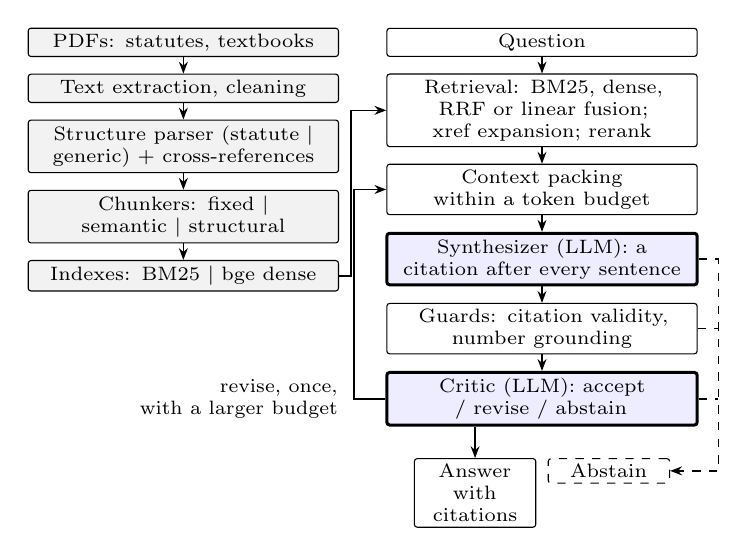
\begin{tikzpicture}[
  font=\scriptsize, node distance=2.1mm,
  box/.style={draw, rounded corners=1pt, align=center, text width=\pipelinebox, inner sep=2pt, fill=white,
    execute at begin node={\hyphenpenalty=10000\exhyphenpenalty=10000}},
  off/.style={box, fill=black!5},
  llm/.style={box, fill=blue!7, line width=1.1pt},
  arr/.style={-{Stealth[length=1.5mm]}, semithick},
  abst/.style={-{Stealth[length=1.5mm]}, semithick, dashed}]
  \node[off] (pdf) {PDFs: statutes, textbooks};
  \node[off, below=of pdf] (ing) {Text extraction, cleaning};
  \node[off, below=of ing] (par) {Structure parser (statute $\mid$ generic) + cross-references};
  \node[off, below=of par] (chk) {Chunkers: fixed $\mid$ semantic $\mid$ structural};
  \node[off, below=of chk] (idx) {Indexes: BM25 $\mid$ bge dense};
  \node[box, right=6mm of pdf] (q) {Question};
  \node[box, below=of q] (ret) {Retrieval: BM25, dense, RRF or linear fusion; xref expansion; rerank};
  \node[box, below=of ret] (pack) {Context packing within a token budget};
  \node[llm, below=of pack] (syn) {Synthesizer (LLM): a citation after every sentence};
  \node[box, below=of syn] (grd) {Guards: citation validity, number grounding};
  \node[llm, below=of grd] (cri) {Critic (LLM): accept / revise / abstain};
  \node[box, below=4mm of cri, xshift=-8.5mm, text width=14mm] (ans) {Answer with citations};
  \node[box, below=4mm of cri, xshift=8.5mm, text width=14mm, dashed] (abs) {Abstain};
  \draw[arr] (pdf) -- (ing); \draw[arr] (ing) -- (par); \draw[arr] (par) -- (chk); \draw[arr] (chk) -- (idx);
  \draw[arr] (q) -- (ret); \draw[arr] (ret) -- (pack); \draw[arr] (pack) -- (syn); \draw[arr] (syn) -- (grd); \draw[arr] (grd) -- (cri);
  \draw[arr] (idx.east) -- ++(1.5mm,0) |- (ret.west);
  \draw[arr] (cri.south -| ans.north) -- (ans.north);
  \coordinate (rail) at ($(cri.east)+(2.5mm,0)$);
  \draw[abst] (syn.east) -- (syn.east -| rail) -- (rail |- abs.east) -- (abs.east);
  \draw[semithick, dashed] (grd.east) -- (grd.east -| rail);
  \draw[semithick, dashed] (cri.east) -- (cri.east -| rail);
  \draw[arr] (cri.west) -- ++(-4mm,0) |- (pack.west);
  \node[font=\scriptsize, anchor=east, align=right] at ($(cri.west)+(-4.8mm,0)$) {revise, once,\\with a larger budget};
\end{tikzpicture}
\caption{Pipeline. Grey: offline ingestion. Blue with a thick border: LLM calls. A guard failure or a revise verdict triggers one revision round. Dashed: abstention paths (the synthesizer finds no answer, or the guards or critic still reject after the revision). Not shown: G5's retrieval-score threshold and the web app's gate, which can abstain before packing. Which components run depends on the system (Table~\ref{tab:generation}).}
\label{fig:arch}
\end{figure}


Fig.~\ref{fig:arch} shows the pipeline; every run records its configuration, its git commit (and whether the working tree had uncommitted changes) and its hardware.

\subsection{Ingestion, Chunking and Retrieval}
After PyMuPDF text extraction, cleaning removes running headers, page numbers, watermarks and the Hindi text of the bilingual Gazette copies.
A statute parser recovers chapters, sections or rules, sub-sections, clauses, provisos and explanations, each with a stable identifier, and resolves internal cross-references (\V{cl.xrefs} in the consumer-law corpus); a generic parser handles the textbooks.
\emph{Fixed} chunkers cut windows of \V{ch.fixed256.size} or \V{ch.fixed512.size} tokens. The \emph{semantic} chunker breaks between sentence or clause units where the bge-small cosine distance exceeds its \V{ch.sem.pct}th percentile.
The \emph{structural} chunker emits one chunk per section or rule, splits it at sub-section and then clause boundaries above \V{ch.struct.max} tokens, merges siblings below \V{ch.struct.min} tokens, keeps each definition as its own chunk, and prefixes the embedded text with its heading path.
BM25 uses a tokenizer that also emits normalized statute references; dense retrieval uses bge-small, -base or -large; hybrids fuse both by RRF ($k=\V{ret.rrfk}$) or a linear combination of min--max normalized scores (dense weight $\alpha=\V{ret.alpha}$).
Optional cross-reference expansion (explored on dev, never selected) and optional reranking of the top \V{ret.rerankn} with the cross-encoder \cmd{ms-marco-MiniLM-L-6-v2} follow.
Ranked chunks are packed in order until the next would exceed the token budget (\V{gen.budget} for the local model, \V{h.budget} for the hosted one), each labeled \cmd{[C$i$]}.

\subsection{Generation and Verification}
The \emph{synthesizer} answers in strict JSON from the passages only, ends every sentence with the label of a supporting passage, copies numbers exactly, and abstains when the passages do not answer.
Two deterministic \emph{guards} follow: \emph{citation validity} (every sentence ends with a citation to a passage in the context) and \emph{number grounding} (every number, in digits or words, including amounts in lakh (one hundred thousand) and crore (ten million), occurs by value in a cited passage).
The \emph{critic}, the same LLM with a fact-checking prompt, sees the question, the cited passages and the answer and returns accept, revise or abstain.
After a guard failure or a revise verdict the synthesizer gets one revision round, with the reasons and a context extended to \V{gen.revbudget} tokens; if that round fails too, the system abstains.
The checks work per sentence, but the system releases or withholds the whole answer.

\section{Experimental Setup}
\label{sec:setup}

% Generated by scripts/paper_tables.py -- do not edit by hand.
\begin{table}[t]
\centering\footnotesize\setlength{\tabcolsep}{2pt}
\begin{tabular}{@{}lrrrrrr@{}}
\toprule
 & & & \multicolumn{2}{c}{Chunks} & \multicolumn{2}{c}{Test Q.} \\ \cmidrule(lr){4-5}\cmidrule(l){6-7}
Collection & Docs & Pages & Struct. & Fix-512 & Ans. & Unans. \\ \midrule
Consumer law & 5 & 77 & 326 & 83 & 68 & 17 \\
CS/AI & 3 & 502 & 1,123 & 492 & 40 & 16 \\
\midrule
\multicolumn{7}{@{}l}{\emph{Served by the web app only (not evaluated)}} \\
CS/AI (app) & 5 & 834 & 1,797 & -- & -- & -- \\
Indian law & 4 & 1,264 & 4,367 & -- & -- & -- \\
Human biology & 1 & 1,298 & 2,089 & -- & -- & -- \\
Physics \& chem. & 4 & 4,258 & 5,485 & -- & -- & -- \\
\bottomrule
\end{tabular}
\caption{Collections. Pages are PDF pages kept after cleaning (selected chapters for textbooks). Struct.\ = structural chunks; Fix-512 = fixed windows. The web app serves the structural chunks of the consumer-law row and of the app rows. Test questions are answerable (Ans.) or unanswerable (Unans.).}
\label{tab:corpus}
\end{table}


\subsection{Collections and Questions}
\emph{Consumer law} is India's Consumer Protection Act, 2019 with its E-Commerce, Commissions, Jurisdiction and Mediation Rules; \emph{CS/AI} is selected chapters of \emph{Dive into Deep Learning}, \emph{Pro Git} and \emph{Open Data Structures} (Table~\ref{tab:corpus}).
We built both question sets automatically with qwen2.5:3b.
Answerable candidates were drafted from provisions sampled by document and by type (definition, factual, procedural, numeric, cross-reference and multi-section), with the source provisions as gold evidence.
A candidate was kept only if it passed seven filters in order: format, no provision numbers, lexical overlap with the source of at most \V{ev.copy}, gold-answer numbers present in the source, an LLM support judgment, no conflict when answered from the source alone, and no near-duplicate.
Unanswerable questions asked about topics outside the corpus or moved an accepted question to another law, state or year; they are plainly out of scope, so a retrieval check that they are not answered by the corpus rejected \V{cl.ev.rcheckfail} of \V{cl.ev.rcheckin} consumer-law candidates (\V{cl.ev.usel} selected).
CS/AI has no cross-reference questions. No person reviewed any generated item.
A question belongs to dev when a salted, truncated SHA-256 hash of its id falls below \V{split.dev}, otherwise to test.
This gives \V{cl.ev.dev.a}+\V{cl.ev.dev.u} (answerable + unanswerable) dev questions for consumer law and \V{cs.ev.dev.a}+\V{cs.ev.dev.u} for CS/AI; Table~\ref{tab:corpus} gives the test counts.
Only two evaluation scripts can obtain test questions, every access is logged, and all parameter tuning used dev. Two later decisions used test results: not running G5 on CS/AI, and the primary family of comparisons below.

\subsection{Retrieval Configurations and Metrics}
On dev we ran \V{cl.grid.n} retrieval configurations for consumer law (four chunkers, BM25, three dense encoders and two hybrids, with and without expansion and reranking) and \V{cs.grid.n} for CS/AI (structural and fixed-512 chunkers only).
The best configuration by dev coverage at \V{gen.budget} tokens, overall and per chunker, went to test with two baselines: naive RAG (fixed-512, dense bge-base) and fixed-512 BM25.
A chunk is relevant to a gold provision when it contains part of the provision's own text, of a descendant, or of an ancestor below chapter level (the \emph{strict} variant drops ancestors).
Besides Recall@$k$ (the share of a question's gold provisions covered by the top $k$ chunks) we report \emph{token-budget coverage} at $b$ tokens: the share of gold provisions covered when ranked chunks are taken in order until the next would exceed $b$.
An answer's \emph{faithfulness} is the share of its sentences (citation tags removed) entailed with probability at least \V{nli.thr} by a single cited passage under \cmd{\V{nli.model}}, taking the maximum over \V{nli.win}-token windows of the passage (stride \V{nli.stride}), so long passages are not truncated; a sentence without a citation counts as unsupported. Because the citation guard rejects exactly such sentences, we also report the share of uncited sentences and the NLI \emph{support of cited sentences} separately.
An answer is \emph{correct} when it entails the gold answer under the same model, or for numeric questions contains every gold number.
\emph{Overall accuracy} counts correct answers and abstentions on unanswerable questions over all questions.

\subsection{Generators and Systems}
The local generator is qwen2.5:3b~\cite{qwen2024qwen25} through Ollama (temperature \V{gen.temp}) on the laptop CPU (\V{hw.cpu}; \V{hw.ram}\,GB of RAM; no GPU).
The hosted generator is \gptoss{}~\cite{openai2025gptoss}, a mixture-of-experts model, through \V{h.provider} (reasoning effort ``\V{h.effort}''), chosen, before any of its results were seen, as the largest general instruction-tuned open-weight model the provider listed.
Table~\ref{tab:generation} defines systems G1--G6 and G2H. G2 uses the dev-best retrieval (structural chunks, dense bge-base on consumer law and bge-small on CS/AI). G3 and G5 are derived from the records of G2 and G4 without new LLM calls.
G5 and G6 were run only on consumer law (G5 lowered accuracy there; G6 is the slowest system). The hosted runs stopped before reaching G4H, the hosted model with guards and critic (on consumer law at the provider's daily quota), so G4H has no results.
\ifcsGtwoHready\else The CS/AI G2H run is incomplete (\V{cs.g2h.done} of \V{cs.gen.n} test questions when this draft was built); its entries read \pend{}.\fi

\subsection{Statistics}
Intervals come from a paired bootstrap over questions (\V{boot.n} resamples, 95\% percentile intervals)~\cite{koehn2004significance,dror2018hitchhiker}; a difference is significant when its interval excludes zero.
A percentile interval for binary accuracy can exclude zero when only \V{prim.cl.G4-G2.acc.loss} questions differ, all in one direction, so an accuracy difference also needs a paired permutation test with $p<\V{stat.alpha}$.
\emph{Released-answer faithfulness} is each system's faithfulness over its own answers; comparing only jointly answered questions would score a stricter system on an easier subset.
A family of \V{prim.m} primary comparisons, fixed after the first draft (when the test results were known), is also tested with paired permutation tests and Holm's correction\ifshowprimary{} (Table~\ref{tab:primary})\fi: structural against naive coverage, and G4 against G2 in released-answer faithfulness and accuracy, on both collections, plus G2H against G2 in accuracy on consumer law.

\section{Results}
\label{sec:results}

\subsection{Retrieval}
\label{sec:res-retrieval}

\begin{figure}[t]
\centering
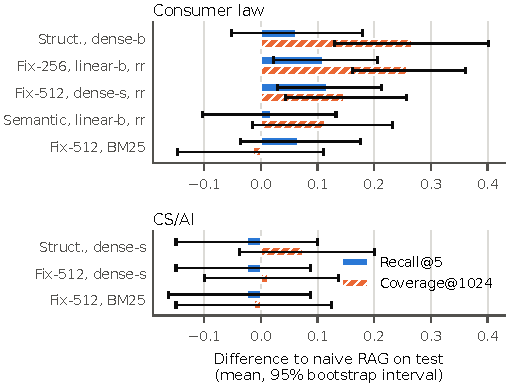
\includegraphics[width=\columnwidth]{figures/retrieval_deltas_ieee.pdf}
\caption{Retrieval on test: paired differences to naive RAG in Recall@5 and coverage at \V{gen.budget} tokens, with 95\% bootstrap intervals. Labels: chunker, retriever and encoder size (s/b); rr = reranking. Naive RAG reaches Recall@5 \V{cl.ret.naive.r5} and coverage \V{cl.ret.naive.cov1024} on consumer law (CS/AI: \V{cs.ret.naive.r5} and \V{cs.ret.naive.cov1024}); the other absolute values are in the extended version~\cite{shukla2026veridexext}.}
\label{fig:retrieval}
\end{figure}

On consumer law (Fig.~\ref{fig:retrieval}), the dev-selected configuration (structural chunks, dense bge-base) raises coverage at \V{gen.budget} tokens from \V{cl.ret.naive.cov1024} to \V{cl.ret.struct-b.cov1024} (\V{cl.ret.struct-b.dcov} \V{cl.ret.struct-b.dcovci}; Holm-adjusted $p=\V{prim.cl.cov.pholm}$; strict relevance: \V{cl.strict.strict.d} \V{cl.strict.strict.dci}), while its Recall@5 difference is \V{cl.ret.struct-b.dr5sig} (\V{cl.ret.struct-b.dr5} \V{cl.ret.struct-b.dr5ci}).
Both use the same encoder, so the difference comes from chunking: structural chunks, which carry their heading path, are short (mean \V{cl.tok.structural} tokens against \V{cl.tok.fixed512}), so a \V{gen.budget}-token budget holds more distinct provisions than the two fixed-512 windows it admits.
Coverage goes with correctness, although both depend on the question type: G2 answers \V{cl.cc.G2.all} of answerable consumer-law questions correctly when every gold provision is in its context and \V{cl.cc.G2.part} otherwise (\V{cl.cc.G2.all.n} and \V{cl.cc.G2.part.n} questions).
Short chunks alone may explain much of the gain: fixed-256 windows reach similar coverage (\V{cl.ret.f256-hyb-rr.dcov} \V{cl.ret.f256-hyb-rr.dcovci}), although that configuration also uses hybrid retrieval and reranking, which raise its latency to \V{cl.ret.f256-hyb-rr.lat}\,ms per query against \V{cl.ret.struct-b.lat}\,ms; we did not test section-aligned and fixed chunks of equal length.
On CS/AI, whose long sections the structural chunker splits more often (\V{cs.split.structural} against \V{cl.split.structural}), no difference is significant, including structural against fixed-512 chunks with the same encoder (coverage \V{cs.dret.struct-s-f512-s.dcov} \V{cs.dret.struct-s-f512-s.dcovci}; not shown in Fig.~\ref{fig:retrieval}).

% Generated by scripts/paper_tables.py -- do not edit by hand.
\begin{table*}[t]
\centering\footnotesize\setlength{\tabcolsep}{3.6pt}
\begin{tabular}{@{}llrrrrrrrrrrr@{}}
\toprule
Coll. & Sys. & Ans. & Faith. & Uncit. & Sup. & Corr. & Overall & Wrong & Refusal & F.\,abst. & Calls & p50 s \\ \midrule
Consumer law & G1 & 0.647 & 0.179 & 0.138 & 0.220 & 0.321 & 0.376 & 38 & 0.882 & 0.221 & 1.05 & 26.7 \\
 & G2 & 0.776 & 0.745 & 0.122 & 0.862 & 0.485 & 0.576 & 34 & 1.000 & 0.029 & 1.00 & 32.5 \\
 & G3 & 0.659 & 0.866 & 0.000 & 0.871 & 0.518 & 0.541 & 27 & 1.000 & 0.176 & 1.00 & 32.5 \\
 & G4 & 0.576 & 0.878 & 0.000 & 0.887 & 0.571 & 0.529 & 21 & 1.000 & 0.279 & 1.98 & 42.3 \\
 & G5 & 0.412 & 0.829 & 0.000 & 0.838 & 0.600 & 0.447 & 14 & 1.000 & 0.485 & 1.25 & 36.9 \\
 & G6 & 0.400 & 0.392 & 0.000 & 0.385 & 0.485 & 0.376 & 18 & 0.941 & 0.515 & 2.31 & 69.0 \\
 & G2H & 0.776 & 0.760 & 0.028 & 0.757 & 0.562 & 0.600 & 30 & 0.882 & 0.059 & 1.00 & 1.2 \\
\midrule
CS/AI & G1 & 0.536 & 0.011 & 0.622 & 0.059 & 0.400 & 0.500 & 18 & 1.000 & 0.250 & 1.00 & 31.6 \\
 & G2 & 0.571 & 0.312 & 0.447 & 0.462 & 0.406 & 0.518 & 19 & 1.000 & 0.200 & 1.00 & 31.1 \\
 & G3 & 0.393 & 0.455 & 0.000 & 0.500 & 0.409 & 0.446 & 13 & 1.000 & 0.450 & 1.00 & 31.1 \\
 & G4 & 0.321 & 0.444 & 0.000 & 0.444 & 0.444 & 0.429 & 10 & 1.000 & 0.550 & 1.77 & 39.5 \\
 & G2H & 0.643 & 0.343 & 0.089 & 0.366 & 0.556 & 0.643 & 16 & 1.000 & 0.100 & 1.00 & 0.6 \\
\bottomrule
\end{tabular}
\caption{Answer quality on the test split. G1 naive RAG (Fix-512, dense-b); G2 dev-best structural retrieval; G3 = G2 with the guards as a release filter (no revision); G4 = G2 + guards + critic, with one revision round; G5 = G4 + dev-tuned score threshold; G6 = Fix-256 hybrid with reranking, guards and critic; G2H = G2 with gpt-oss-120b (others: qwen2.5:3b). Ans.\ = share answered; Faith.\ = released-answer faithfulness (mean over answers); Uncit.\ = share of released sentences without a citation and Sup.\ = NLI support of cited sentences (both pooled over sentences, so they do not combine into Faith.); Corr.\ = correct among answered answerable questions (the accuracy of released answers); Wrong = released answers judged incorrect; F.\,abst.\ = false abstention; Calls = mean LLM calls per question (critic, revision and JSON-repair calls included); p50 s = median latency. Metrics: \S\ref{sec:setup}; citation precision and recall: Table~\ref{tab:genextra}.}
\label{tab:generation}
\end{table*}

% Generated by scripts/paper_tables.py -- do not edit by hand.
\begin{table}[t]
\TabCaption{tab:bootstrap}{Main paired differences on the test split with 95\% bootstrap intervals (\V{boot.n} resamples over questions)}{Released faithfulness = faithfulness over the answers each system releases (uncited sentences count as unsupported); support of cited sentences = NLI support among released sentences that carry a citation. Bold = interval excludes 0 (a bound at 0.000 counts as including 0); for overall accuracy, bold also requires a paired permutation test to give $p<0.05$ (uncorrected), and $^\dagger$ marks an interval that excludes 0 without it (few questions differ). -- = not computed. Faithfulness on jointly answered questions, correct refusal and further pairs: \ExtRef{Table}{tab:bootstrap-full}.}%
\centering\scriptsize\setlength{\tabcolsep}{2.2pt}
\begin{tabular}{@{}lrrr@{}}
\toprule
\makecell[l]{Comparison\\(what changes)} &\makecell[r]{$\Delta$ Released\\faithfulness} & \makecell[r]{$\Delta$ Support of\\cited sentences} & \makecell[r]{$\Delta$ Overall\\accuracy} \\ \midrule
\multicolumn{4}{@{}l}{\emph{Consumer law}} \\
\makecell[l]{G2$-$G1\\{retrieval}} & \makecell[r]{\textbf{+0.566}\\{\textbf{[0.420, 0.715]}}} & \makecell[r]{\textbf{+0.642}\\{\textbf{[0.491, 0.781]}}} & \makecell[r]{\textbf{+0.200}\\{\textbf{[0.094, 0.306]}}} \\[1pt]
\makecell[l]{G3$-$G2\\{guards}} & \makecell[r]{\textbf{+0.121}\\{\textbf{[0.048, 0.191]}}} & \makecell[r]{+0.009\\{[$-$0.012, 0.042]}} & \makecell[r]{$-$0.035\\{[$-$0.082, 0.000]}} \\[1pt]
\makecell[l]{G4$-$G2\\{guards + critic}} & \makecell[r]{\textbf{+0.133}\\{\textbf{[0.053, 0.214]}}} & \makecell[r]{+0.025\\{[$-$0.019, 0.081]}} & \makecell[r]{$-$0.047$^\dagger$\\{[$-$0.094, $-$0.012]}} \\[1pt]
\makecell[l]{G4$-$G3\\{critic + revision}} & \makecell[r]{+0.011\\{[$-$0.022, 0.054]}} & \makecell[r]{+0.016\\{[$-$0.021, 0.060]}} & \makecell[r]{$-$0.012\\{[$-$0.047, 0.024]}} \\[1pt]
\makecell[l]{G5$-$G4\\{threshold}} & \makecell[r]{\textbf{$-$0.049}\\{\textbf{[$-$0.106, $-$0.014]}}} & -- & \makecell[r]{\textbf{$-$0.082}\\{\textbf{[$-$0.153, $-$0.035]}}} \\[1pt]
\makecell[l]{G2H$-$G2\\{generator, budget}} & \makecell[r]{+0.015\\{[$-$0.121, 0.150]}} & \makecell[r]{$-$0.104\\{[$-$0.219, 0.007]}} & \makecell[r]{+0.024\\{[$-$0.071, 0.129]}} \\[1pt]
\midrule
\multicolumn{4}{@{}l}{\emph{CS/AI}} \\
\makecell[l]{G2$-$G1\\{retrieval}} & \makecell[r]{\textbf{+0.301}\\{\textbf{[0.156, 0.462]}}} & \makecell[r]{\textbf{+0.403}\\{\textbf{[0.184, 0.615]}}} & \makecell[r]{+0.018\\{[$-$0.089, 0.125]}} \\[1pt]
\makecell[l]{G3$-$G2\\{guards}} & \makecell[r]{\textbf{+0.142}\\{\textbf{[0.059, 0.263]}}} & \makecell[r]{+0.038\\{[0.000, 0.101]}} & \makecell[r]{$-$0.071$^\dagger$\\{[$-$0.143, $-$0.018]}} \\[1pt]
\makecell[l]{G4$-$G2\\{guards + critic}} & \makecell[r]{+0.132\\{[$-$0.023, 0.321]}} & \makecell[r]{$-$0.017\\{[$-$0.185, 0.167]}} & \makecell[r]{$-$0.089$^\dagger$\\{[$-$0.161, $-$0.018]}} \\[1pt]
\makecell[l]{G4$-$G3\\{critic + revision}} & \makecell[r]{$-$0.010\\{[$-$0.149, 0.140]}} & \makecell[r]{$-$0.056\\{[$-$0.220, 0.120]}} & \makecell[r]{$-$0.018\\{[$-$0.054, 0.000]}} \\[1pt]
\makecell[l]{G2H$-$G2\\{generator, budget}} & \makecell[r]{+0.030\\{[$-$0.172, 0.242]}} & \makecell[r]{$-$0.096\\{[$-$0.306, 0.153]}} & \makecell[r]{+0.125$^\dagger$\\{[0.018, 0.232]}} \\[1pt]
\bottomrule
\end{tabular}
\TabNotes
\end{table}

\ifshowprimary% Generated by scripts/paper_tables.py -- do not edit by hand.
\begin{table*}[t]
\TabCaption{tab:primary}{Primary comparisons with paired permutation tests (10,000 permutations) and Holm's correction across the 7 tests}{This family was fixed after the first draft, as a robustness check of the bootstrap intervals. Discord.\ = questions only the first system got right / only the second.}%
\centering\footnotesize\setlength{\tabcolsep}{5pt}
\begin{tabular}{@{}llrrrr@{}}
\toprule
Coll. & Comparison & $\Delta$ & $p$ & $p_{\mathrm{Holm}}$ & Discord. \\ \midrule
Cons.\ law & coverage@1024, structural $-$ naive & +0.267 & 0.0003 & 0.0021 & -- \\
CS/AI & coverage@1024, structural $-$ naive & +0.075 & 0.3364 & 0.6727 & -- \\
Cons.\ law & released faithfulness, G4 $-$ G2 & +0.133 & 0.0023 & 0.0138 & -- \\
Cons.\ law & overall accuracy, G4 $-$ G2 & $-$0.047 & 0.1214 & 0.3642 & 0/4 \\
Cons.\ law & overall accuracy, G2H $-$ G2 & +0.024 & 0.8136 & 0.8136 & 10/8 \\
CS/AI & released faithfulness, G4 $-$ G2 & +0.132 & 0.0830 & 0.3320 & -- \\
CS/AI & overall accuracy, G4 $-$ G2 & $-$0.089 & 0.0600 & 0.3000 & 0/5 \\
\bottomrule
\end{tabular}
\TabNotes
\end{table*}
\fi

\subsection{Generation and Faithfulness}
\label{sec:res-generation}

The retrieval change gives the largest gain on test (Tables~\ref{tab:generation} and~\ref{tab:bootstrap}): G2 improves on naive RAG in released-answer faithfulness and cited-sentence support on both collections, and in overall accuracy on consumer law only (\V{cl.boot.G2-G1.acc} \V{cl.boot.G2-G1.accci}).

Guards alone (G3) and guards with the critic (G4) raise released-answer faithfulness over G2 on consumer law (\V{cl.rel.G3-G2} \V{cl.rel.G3-G2ci}; \V{cl.rel.G4-G2} \V{cl.rel.G4-G2ci}, Holm-adjusted $p=\V{prim.cl.G4-G2.rel.pholm}$), but the metric counts uncited sentences as unsupported and the citation guard withholds exactly the answers that contain them (\V{cl.sent.G2.uncited} of G2's released sentences on consumer law, \V{cs.sent.G2.uncited} on CS/AI).
Among cited sentences, NLI support does not change significantly on either collection (consumer law: \V{cl.cit.G4-G2} \V{cl.cit.G4-G2ci}), and the critic with its revision round adds nothing measurable over the guard filter (G4$-$G3: \V{cl.rel.G4-G3} \V{cl.rel.G4-G3ci}) while nearly doubling the LLM calls.
The verifier therefore mainly enforces the citation format and shows no measurable ability to detect cited but unsupported content, in line with weak self-critique by small models~\cite{huang2024selfcorrect}.
Filtering does reduce wrong answers: on consumer law G4 releases \V{cl.sent.G4.wrong} answers judged incorrect against \V{cl.sent.G2.wrong} for G2, at the price of \V{cl.sent.G4.correct} correct answers against \V{cl.sent.G2.correct}.
The overall-accuracy differences of G4 to G2 rest on \V{prim.cl.G4-G2.acc.loss} (consumer law) and \V{prim.cs.G4-G2.acc.loss} (CS/AI) questions that G2 got right and G4 did not, with none in the other direction; the permutation tests give $p=\V{prim.cl.G4-G2.acc.p}$ and $p=\V{prim.cs.G4-G2.acc.p}$, not significant even before correction.
G2 and G4 refuse every unanswerable question, but these are easy; naive RAG already refuses \V{cl.gen.G1.refusaln} of \V{cl.gen.nunans} and \V{cs.gen.G1.refusaln} of \V{cs.gen.nunans}.
G6, built on the configuration with the best dev Recall@5, is far worse than G4 (released-answer faithfulness \V{cl.rel.G6-G4} \V{cl.rel.G6-G4ci}).

A larger generator helps, if at all, on the textbooks.
G2H replaces qwen2.5:3b by \gptoss{}, which also brings a larger context budget, a larger output limit and hidden reasoning. On consumer law its differences to G2 have wide intervals (Table~\ref{tab:bootstrap}), so the data neither detect a difference nor show that there is none.
On CS/AI it raises accuracy by \V{cs.boot.G2H-G2.acc} \V{cs.boot.G2H-G2.accci}: it abstains less on answerable questions (\V{cs.gen.G2H.falseabspct} against \V{cs.gen.G2.falseabspct}) and more of its answers are correct. The gain rests on \V{sec.cs.G2H-G2.acc.win} questions only G2H got right against \V{sec.cs.G2H-G2.acc.loss} only G2 got right, and a paired permutation test, outside the corrected family, gives $p=\V{sec.cs.G2H-G2.acc.p}$; released-answer faithfulness does not change significantly.
On consumer law G2H cites several passages in one sentence more often (\V{cl.sent.G2H.multi} of \V{cl.sent.G2H.n} sentences against \V{cl.sent.G2.multi} of \V{cl.sent.G2.n}), which a single-passage judge cannot credit; its cited-sentence support changes by \V{cl.cit.G2H-G2} \V{cl.cit.G2H-G2ci}.
Run on the provider's hardware, it is much faster than the local model on the laptop CPU (median \V{cl.gen.G2H.p50}\,s against \V{cl.gen.G2.p50}\,s on consumer law).

\ifshowdomain
On the textbooks, faithfulness is lower at every stage (G2: \V{cs.gen.G2.faith} against \V{cl.gen.G2.faith}), largely because the small model leaves \V{cs.sent.G2.uncited} of its CS/AI sentences uncited; G4 then withholds \V{cs.gen.G4.falseabspct} of the answerable CS/AI questions (the guard filter alone, G3: \V{cs.gen.G3.falseabspct}).
\fi

\subsection{Abstention}
\label{sec:res-abstention}

\ifshowselective
\begin{figure}[t]
\centering
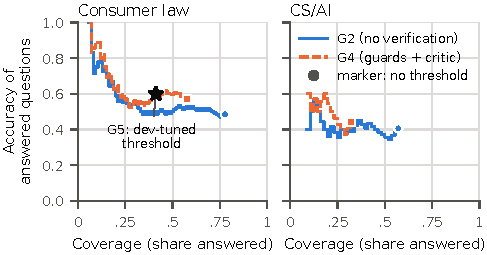
\includegraphics[width=\columnwidth]{figures/selective.pdf}
\caption{Accuracy of released answers against coverage (share of questions answered) when G2 and G4 also abstain below a top-1 retrieval-score threshold swept over the test scores (descriptive; points with at least five answered questions). Circle (G2) and square (G4) at the right end: no threshold. Star: G5, i.e.\ G4 with the threshold tuned on dev.}
\label{fig:selective}
\end{figure}
\fi

G5 abstains before any LLM call when the top-1 dense cosine falls below a threshold (\V{abs.thr}) tuned on dev for the abstention F1 of the threshold alone, although G4 already refuses every unanswerable question.
On test it abstained before generation on \V{cl.gen.G5.lowretrievalscore} questions, raised false abstention from \V{cl.gen.G4.falseabspct} to \V{cl.gen.G5.falseabspct}, lowered released-answer faithfulness by \V{cl.rel.G5-G4} \V{cl.rel.G5-G4ci} and changed accuracy relative to G4 by \V{cl.boot.G5-G4.acc} \V{cl.boot.G5-G4.accci} (all \V{sec.cl.G5-G4.acc.loss} discordant questions favor G4; permutation $p=\V{sec.cl.G5-G4.acc.p}$).
Besides the small dev set, the tuning objective explains this: the score separates answerable from unanswerable test questions well (area under the ROC curve \V{cl.ret.struct-b.auroc}), but G4 left no unanswerable questions for it to catch.
\ifshowselective In the descriptive sweep of Fig.~\ref{fig:selective}, at\else In a descriptive sweep of the threshold, at\fi{} G4's answer rate (\V{cl.sel.G4.cov0}), G2 with a score threshold reaches an accuracy of released answers of \V{cl.sel.G2.atG4}, against \V{cl.sel.G4.acc0} for G4; abstaining at random would keep G2's \V{cl.sel.G2.acc0}. The verifier thus selects somewhat better than a retrieval-score rule at an equal answer rate, a descriptive comparison we did not test.

\ifshowerrors% Generated by scripts/paper_tables.py -- do not edit by hand.
\begin{table}[t]
\centering\footnotesize\setlength{\tabcolsep}{4pt}
\begin{tabular}{@{}lrrr@{}}
\toprule
Category & Cons.\ law & CS/AI & Total \\ \midrule
Retrieval miss & 2 & 3 & 5 \\
Chunk boundary & 0 & 0 & 0 \\
Synthesis error & 4 & 0 & 4 \\
Verifier false reject & 0 & 4 & 4 \\
Verifier false accept & 0 & 0 & 0 \\
Evaluation artefact & 5 & 2 & 7 \\
\midrule
Sampled failures & 11 & 9 & 20 \\
\bottomrule
\end{tabular}
\caption{Error categories of 20 G4 test failures (of \V{cl.err.nfail} consumer-law and \V{cs.err.nfail} CS/AI failures), sampled with seed \V{err.seed} in proportion to the failures per collection.}
\label{tab:errors}
\end{table}
\fi

\subsection{Error Analysis}
\label{sec:res-errors}

We sampled \V{err.n} G4 test failures (an answerable question answered incorrectly or withheld, or an unanswerable one answered), \V{cl.err.nsample} on consumer law and \V{cs.err.nsample} on CS/AI in proportion to their failures.
Rule-based pre-labels were checked against each record, and the final labels were assigned with AI assistance (\V{err.agree} of \V{err.n} pre-labels kept).
The largest group\ifshowerrors{} in Table~\ref{tab:errors}\fi, \emph{evaluation artifacts} (\V{err.evalartifact}), are not system errors: correct answers that the NLI judge does not entail (code, a formula, a short noun phrase), one gold answer that contradicts its source and one ambiguous question.
\emph{Retrieval misses} (\V{err.retrievalmiss}) ranked the gold provision below what fit in the context; in \emph{synthesis errors} (\V{err.synthesiserror}) the evidence was in the context but the answer was wrong or did not answer.
All \emph{verifier false rejects} (\V{err.verifierfalsereject}) are on CS/AI: correct answers withheld, three because a sentence lacked its citation tag and one after a critic revision request.

\ifshowdeployment\section{Deployment}
\label{sec:deploy}

The public assistant is a static site on GitHub Pages with a proxy on the Cloudflare Workers free plan, free only within the model provider's free-tier quotas. A Web Worker in the browser embeds the question with bge-small-en-v1.5 and searches \V{lib.passages} int8 passage vectors (\V{lib.vecgz}\,MB gzip) in \V{web.embed.p50}\,ms and \V{web.search.p50}\,ms per question on the laptop (medians over \V{web.nq} dev questions).
No answer-quality number in this paper measures the app: it retrieves with dense bge-small and a similarity gate only, three of its collections are unevaluated, its generator (\gptoss{}) was evaluated only without guards and critic, and its ``verified'' label comes from the guards and critic and does not involve the NLI judge.
\fi
\section{Limitations}
\label{sec:limitations}

The test splits hold \V{cl.ev.test.n} and \V{cs.ev.test.n} questions, so intervals are wide and several comparisons are inconclusive: they neither show nor exclude a difference. Some significant differences rest on a handful of questions.
The same small model that answers the questions also generated and filtered them, from one or two source provisions with those provisions as gold evidence; this may favor the structural chunker and push the generator comparison toward no difference.
No item was reviewed by a person: the error analysis found a wrong gold answer and an ambiguous question, and \V{cs.ev.test.passageref} of the \V{cs.ev.test.a} answerable CS/AI test questions refer to ``the passage'' or ``the text'', which a user never sees. The unanswerable questions are plainly out of scope, so refusal rates say little.
Faithfulness and correctness rest on one NLI model with a fixed threshold that needs a single cited passage to entail a sentence; we did not validate it against human labels or a second judge, and sampling failures reveals only its false negatives. The error categories were assigned with AI assistance in a single pass without a second annotator.
Only one local and one hosted generator were tested; the hosted one also changes the budgets and reasoning and was tested without guards and critic. The primary family was fixed after the first draft and does not include the CS/AI generator comparison.
Quantized local inference and hosted APIs are not guaranteed to be bit-reproducible, and the test runs were made from working trees with uncommitted changes whose diffs were not recorded.

\section{Conclusion}
\label{sec:conclusion}

On held-out questions, structure-aware chunking increased the share of gold evidence that fits in the generator's context for statutes; for textbooks the difference was not significant.
Verification behaved as a filter that mainly enforces citation format, with no measurable change in the support of cited sentences, and a larger hosted generator made no detectable difference on the statutes and gave an unconfirmed accuracy gain on the textbooks.
Of \V{err.n} sampled failures, \V{err.evalartifact} were evaluation artifacts.
Comparing such systems on small margins needs human-checked test sets, validated judges and verifiers tested on content as well as format.

\section*{Acknowledgment}

In developing this work, I used Anthropic's Claude and Claude Code to assist with writing the core algorithmic scripts and with drafting and editing the text and tables of this paper. I manually inspected and verified every segment of the generated code along with all reported figures, and I assume full responsibility for the accuracy of the findings.


\bibliographystyle{IEEEtran}
% references_ieee.bib is ../references.bib without the urls IEEE style omits (scripts/paper_tables.py)
\bibliography{references_ieee}

\end{document}
